\documentclass[12pt,a4paper]{article}%[a4paper,portuguese,12pt,pdftex]{article} %article
\usepackage{ucs}
\usepackage{amsfonts}		 		% usar fontes p/ REAL,IMAGINARIO,etc
\usepackage{indentfirst}			% espacamento no 1o. paragrafo
\usepackage[utf8x]{inputenc} 
\usepackage{amssymb,amsmath}			% pacote simbolos e matematico AMS
\usepackage{textcomp}
\usepackage{natbib}				% estilo de citacao no texto
\usepackage{wasysym}
\usepackage{fancyhdr}
\renewcommand{\baselinestretch}{1.5}		% espaco entre linhas
\topmargin -1cm					% margem superior
\oddsidemargin 0.5cm				% margem esquerda
\textwidth 15cm					% largura da pagina
\textheight 23.7cm				% altura da pagina
\usepackage{color}
\usepackage{lscape}
\usepackage{graphicx}
\usepackage{epsfig}

\title{Learning velocity fields from sparse data using Gaussian Process}
\author{}

\begin{document}

\section{Building a velocity field with one observation}
Here, the effect of a single observation is observed. Three different kernels are tested: 
a divergence-free kernel, a curl-free kernel and an isotropic squared-exponential kernel 
(Figure \ref{one_obs}). 

\begin{figure}
\centering\includegraphics[width=24pc]{plots/one_obs.png}
\caption{Velocity fields constructed from one observation (red vectors) considering 
different kernel functions. In all of them, the decorrelation length was $\sigma=0.1$.} 
\label{one_obs}
\end{figure}

\newpage

\section{Building a velocity field with two observations}
Here, the combined effect of two observations in the construction of a velocity field using 
the divergence-free kernel is explored. Figures \ref{2-vec-45}, \ref{2-vec-90}, and \ref{2-vec-180} 
show the construction of velocity fields considering differences in the relative position of 
the observations, intensity and direction.

\begin{figure}
\centering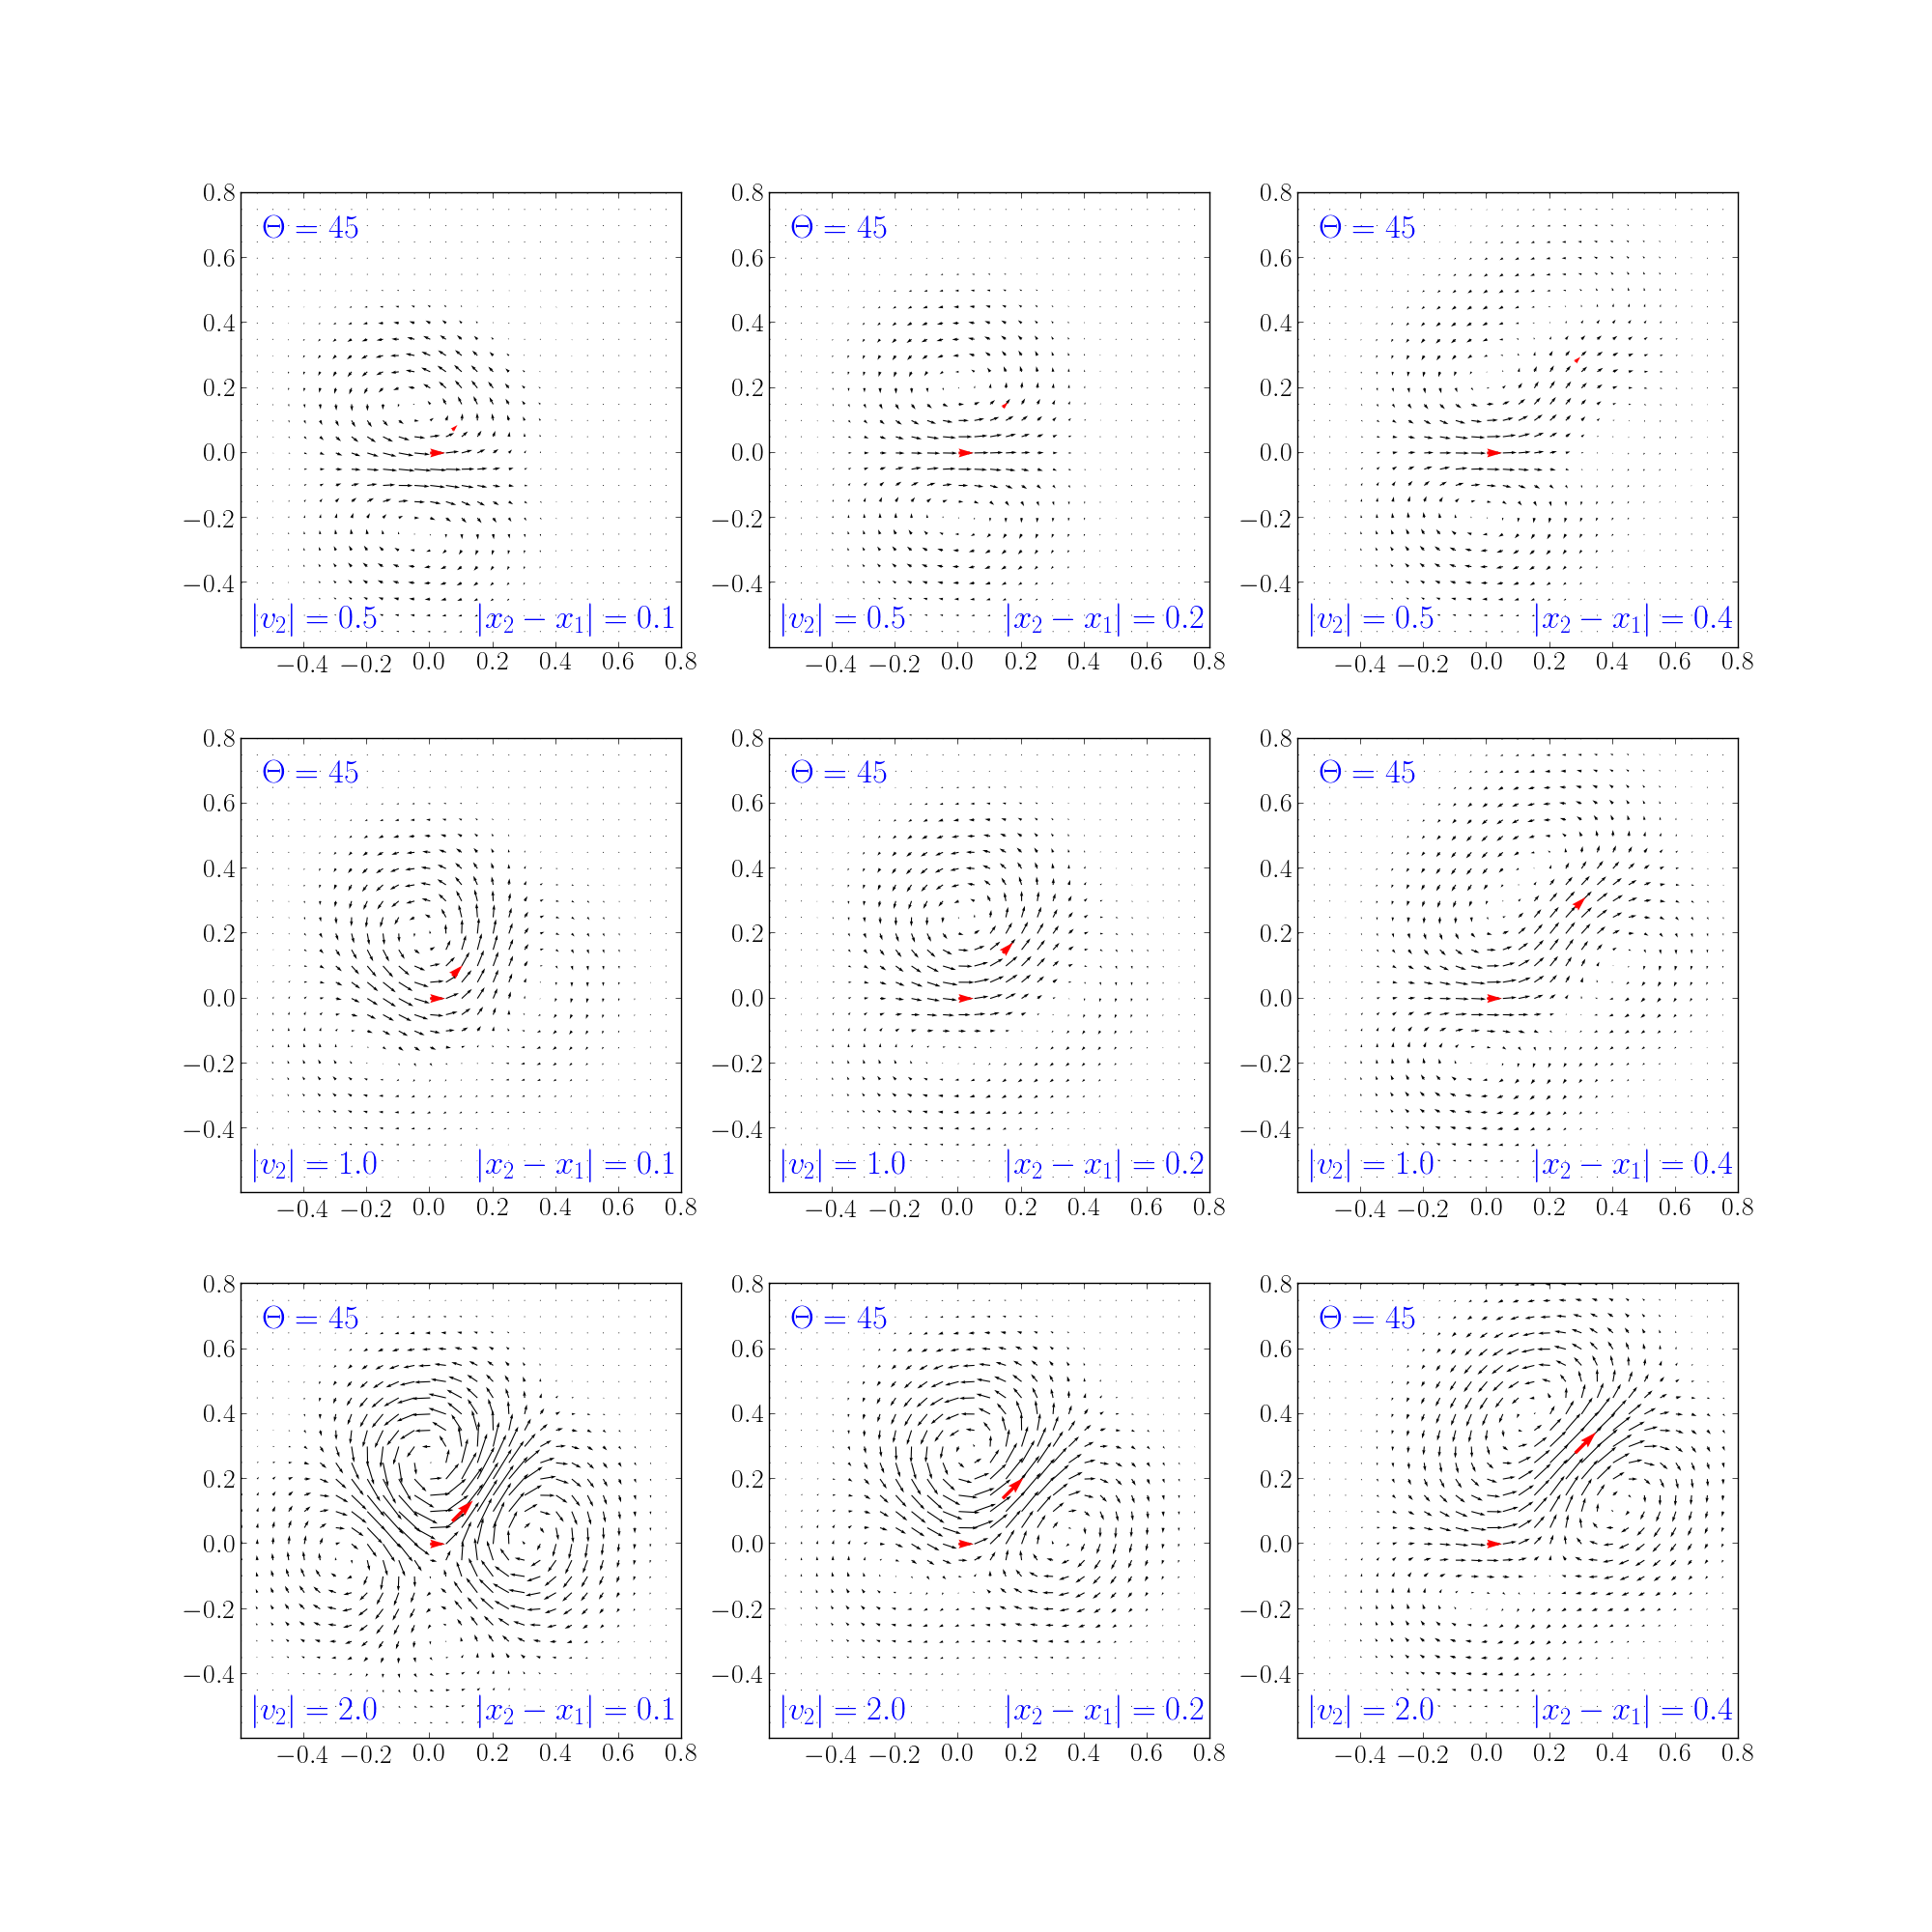
\includegraphics[width=36pc]{plots/2_vectors_angle_45.png}
\caption{Velocity fields constructed from two observations (red vectors). 
In each construction,  different distances between observations ($|x_2 - x_1|$) 
and different absolute velocities of one observation ($|v_2|$) were considered. 
For all 6 cases, the difference in the velocity direction is $\Theta=45^o$. }
\label{2-vec-45}
\end{figure}

\begin{figure}
\centering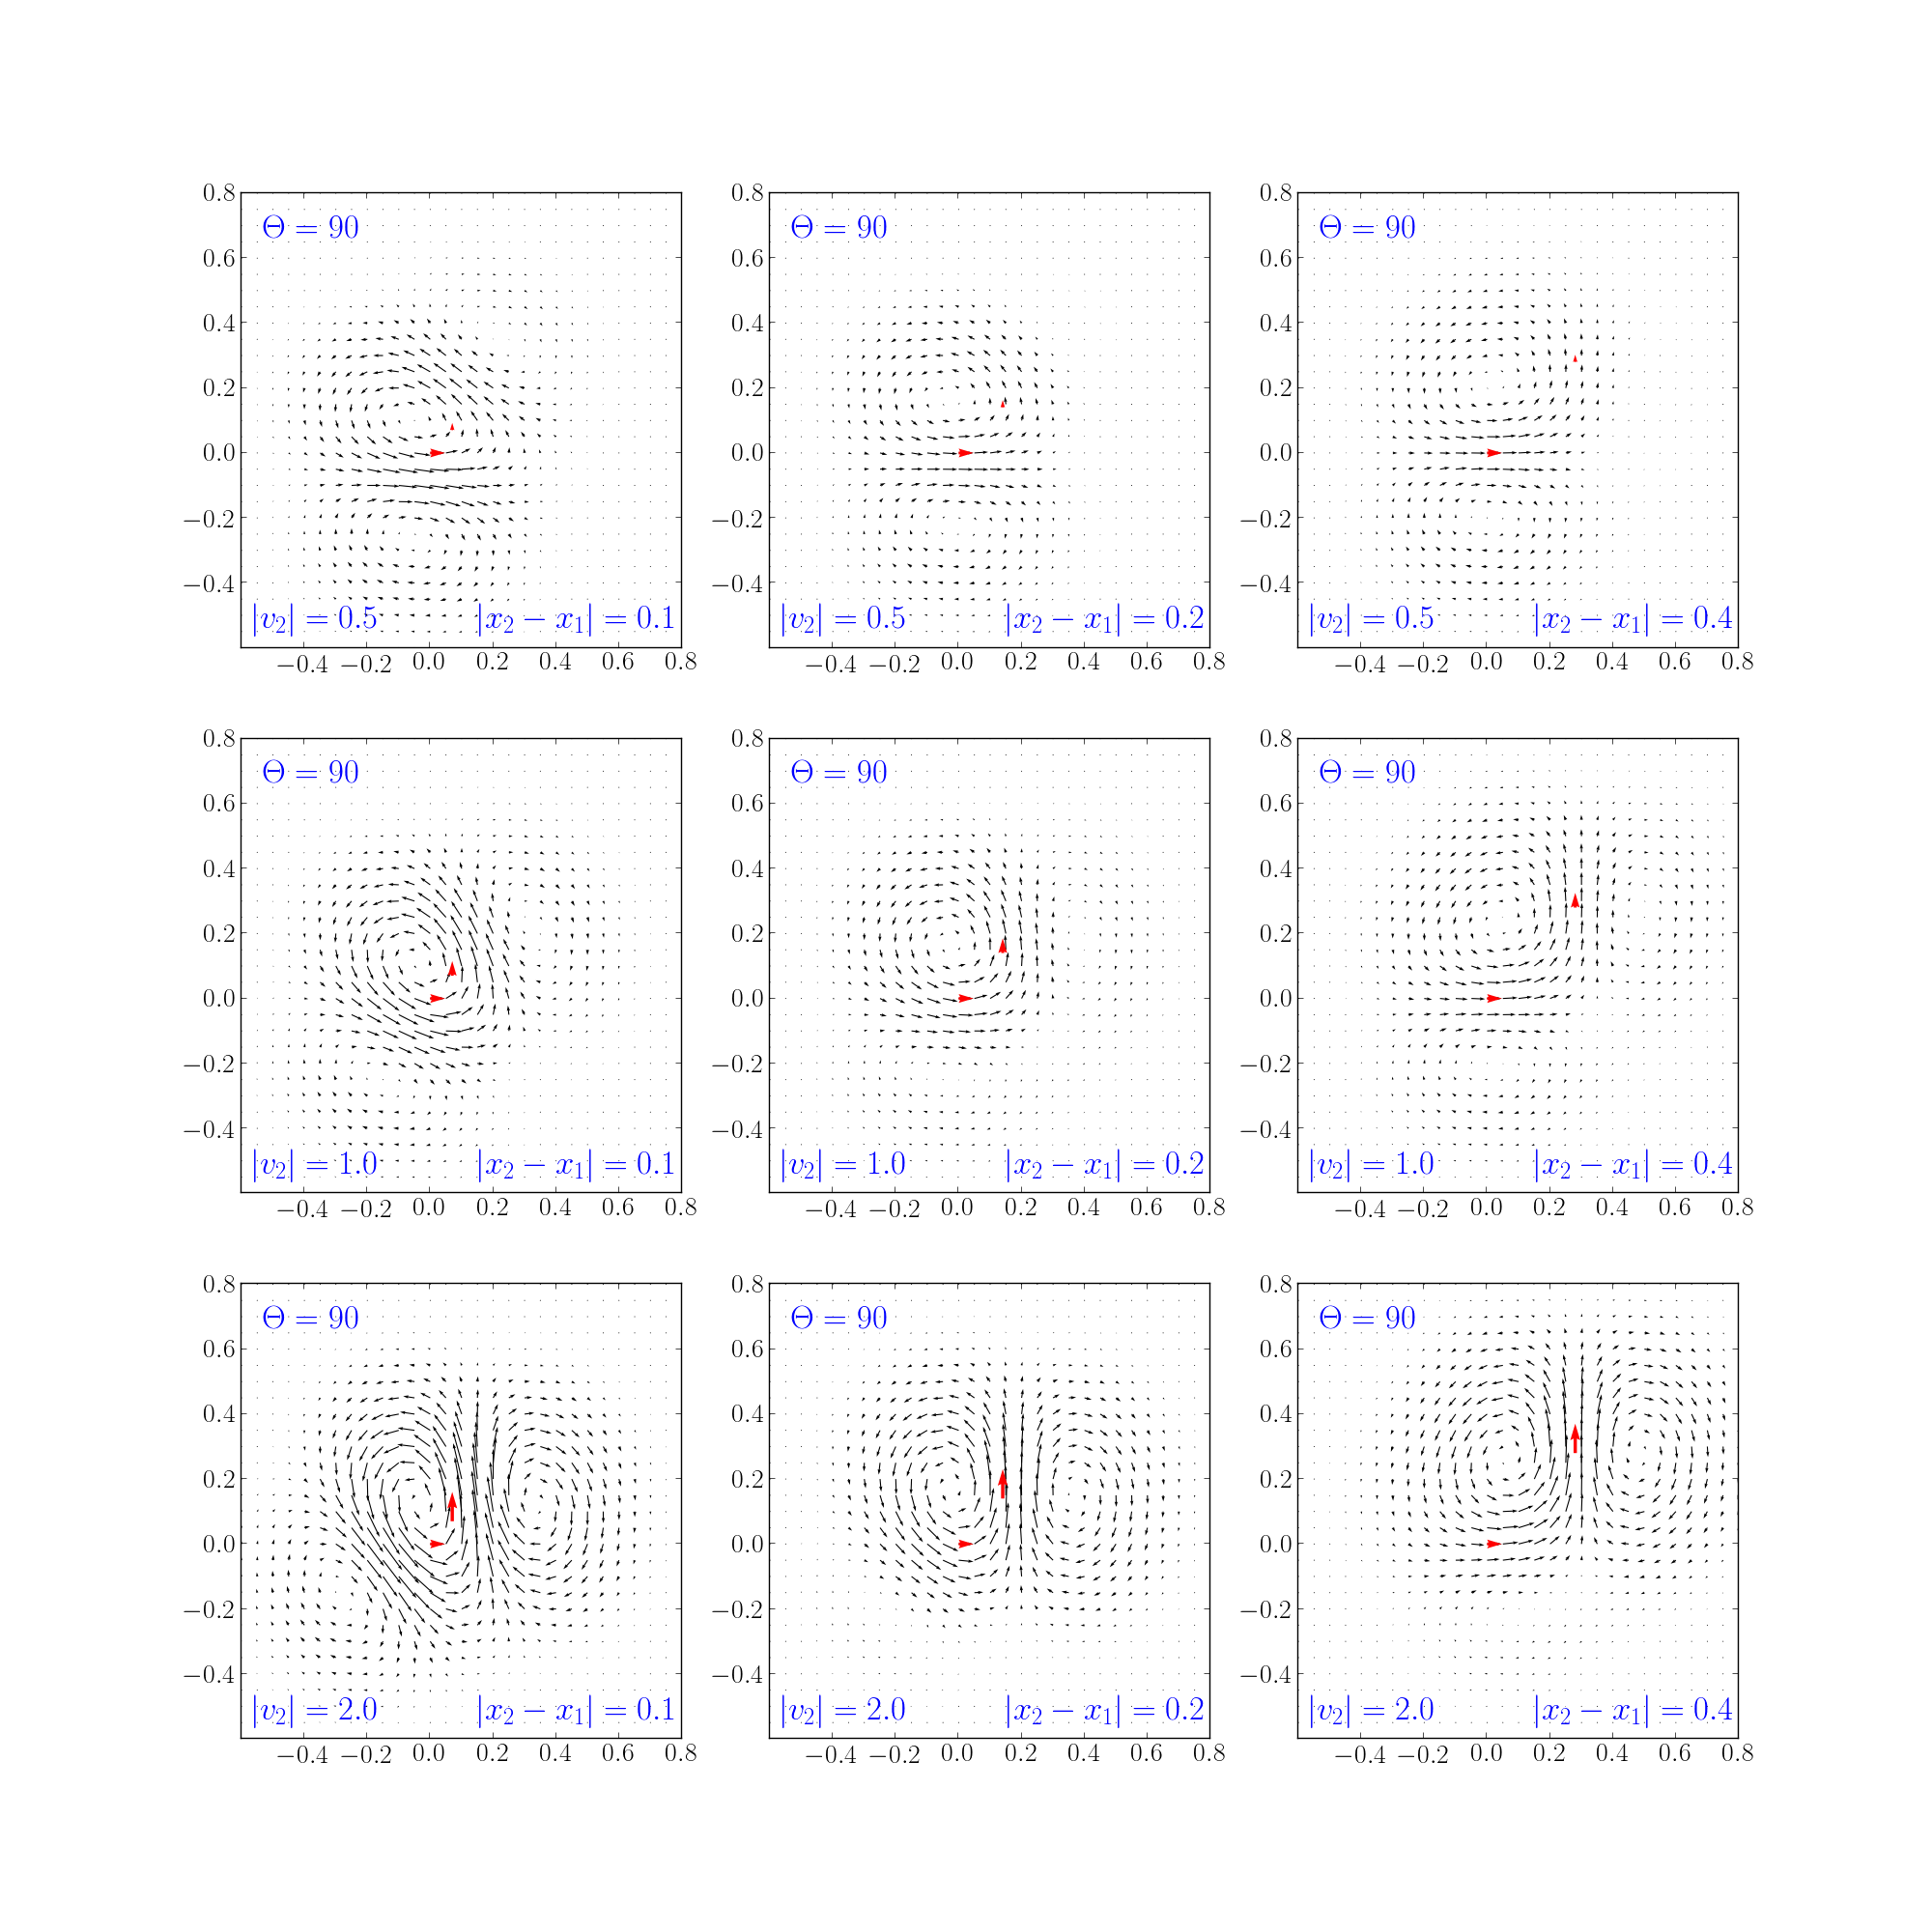
\includegraphics[width=36pc]{plots/2_vectors_angle_90.png}
\caption{Velocity fields constructed from two observations (red vectors). 
In each construction,  different distances between observations ($|x_2 - x_1|$) 
and different absolute velocities of one observation ($|v_2|$) were considered. 
For all 6 cases, the difference in the velocity direction is $\Theta=90^o$. }
\label{2-vec-90}
\end{figure}

\begin{figure}
\centering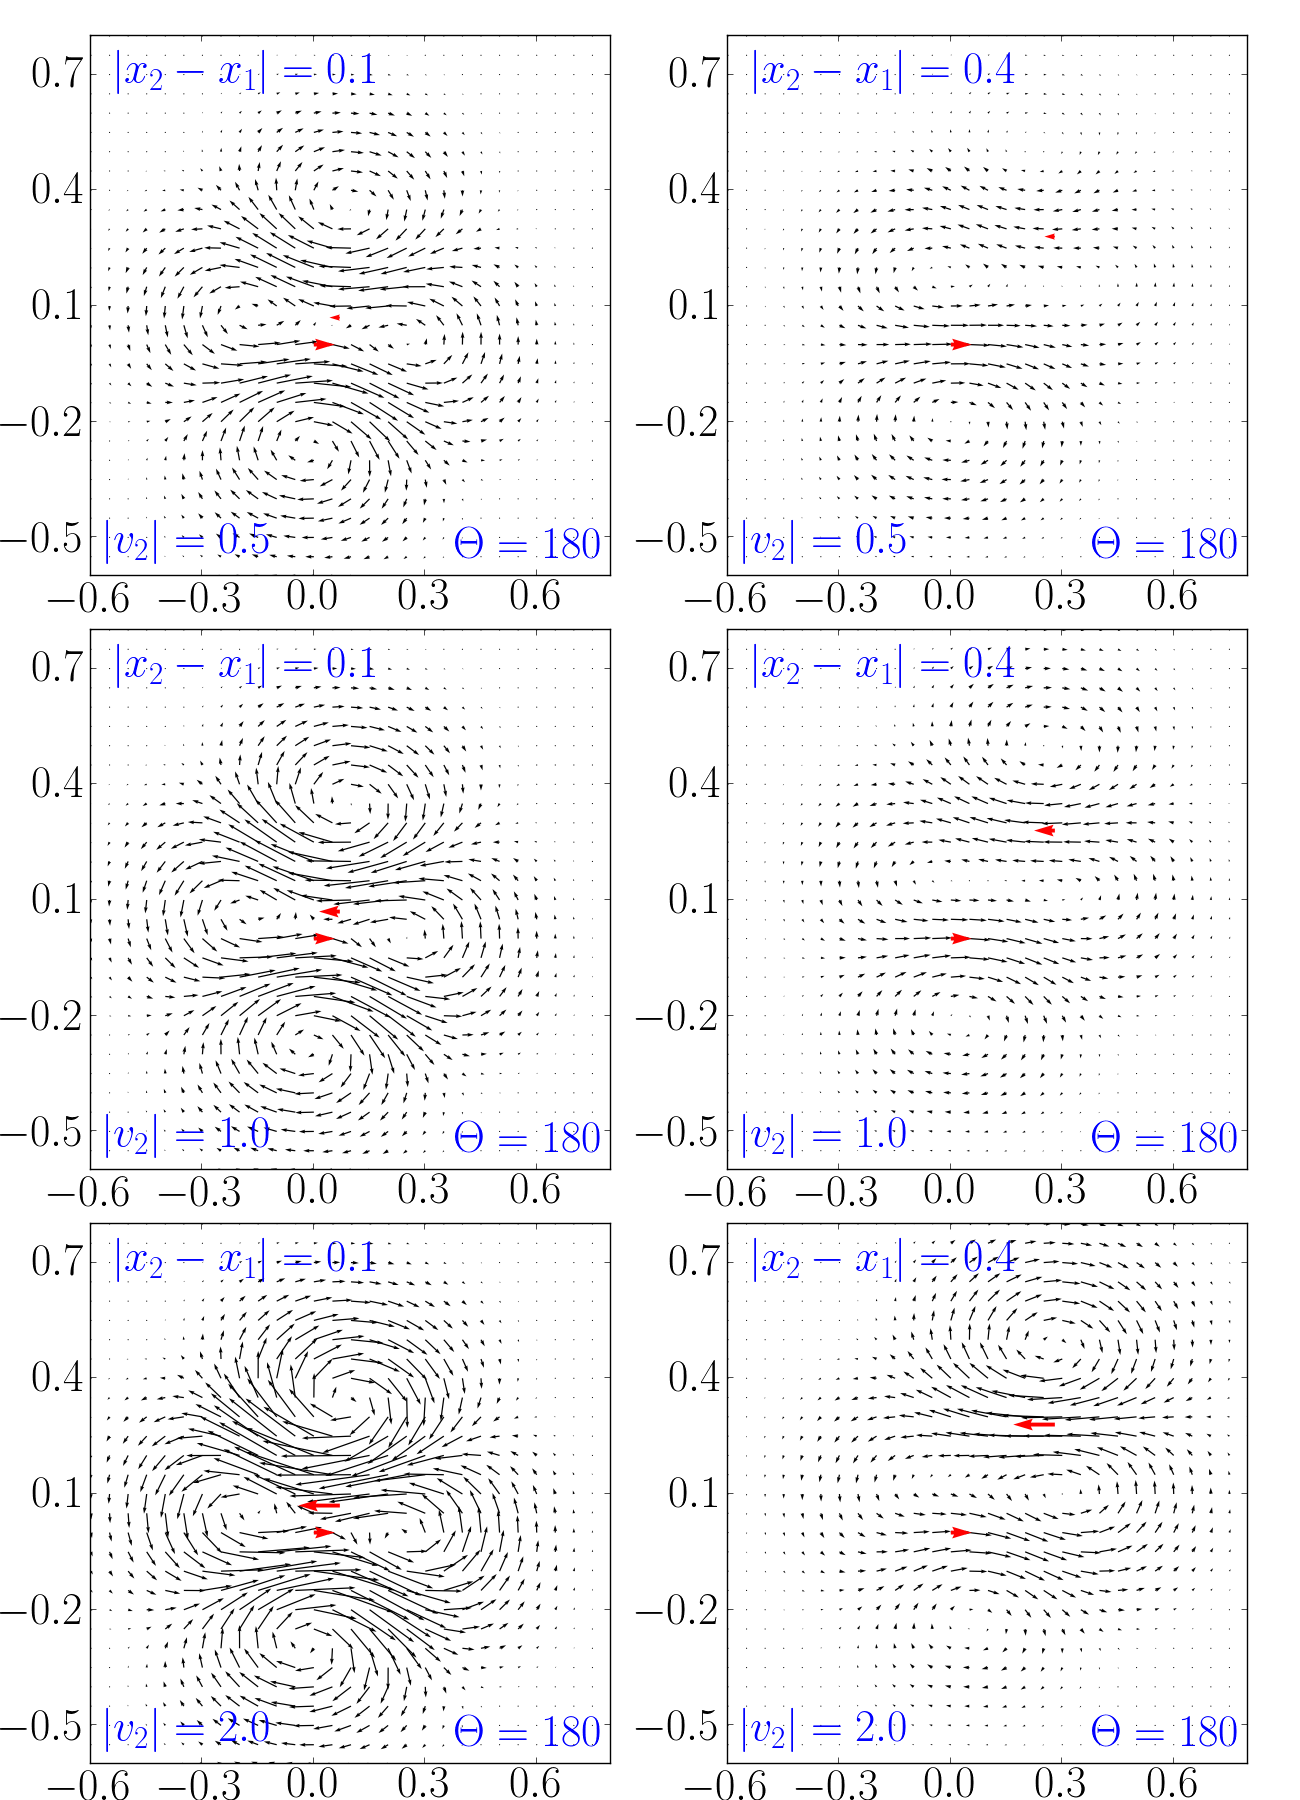
\includegraphics[width=36pc]{plots/2_vectors_angle_180.png}
\caption{Velocity fields constructed from two observations (red vectors). 
In each construction,  different distances between observations ($|x_2 - x_1|$) 
and different absolute velocities of one observation ($|v_2|$) were considered. 
For all 6 cases, the difference in the velocity direction is $\Theta=180^o$. }
\label{2-vec-180}
\end{figure}

\newpage
\section{Reconstruction of a non-divergent velocity field}

In this exercise, the non-divergent kernel was applied to reconstruct 
a non-divergent velocity field. The original velocity field (Figure \ref{div-free-field}) 
was created by taking the curl of a 2D Gaussian surface. For the reconstruction, 3 
different values of the decorrelation length ($\sigma$) were tested (0.1, 0.3 and 0.5). 
For comparison, a fourth reconstruction was carried out using the isotropic squared 
exponential kernel with $\sigma = 0.5$. The results of this exercise are presented on the 
following figures.


\begin{figure}
\centering\includegraphics[width=20pc]{plots/non-div-field.png}
\caption{Original velocity field.}
\label{div-free-field}
\end{figure}



\begin{figure}
\noindent\includegraphics[width=36pc]{plots/Reconstructed-Velocity.png}
\caption{Reconstructed velocity fields considering different decorrelation 
distances ($\sigma$) or kernels. Top-left, top-right and bottom-left: 
divergence-free kernel with $\sigma=0.1$, $\sigma=0.3$, and $sigma=0.5$, 
respectively. Bottom-right: isotropic squared-exponential kernel with 
$\sigma=0.5$. The red dots indicate the location of the observations.}
\label{vel_vectors}
\end{figure}

\begin{figure}
\noindent\includegraphics[width=36pc]{plots/Velocity-Error.png}
\caption{Difference between the reconstructed velocity fields from Figure 
\ref{vel_vectors}} and the original velocity field (Figure \ref{div-free-field}).

\label{vel_errors}
\end{figure}


\begin{figure}
\noindent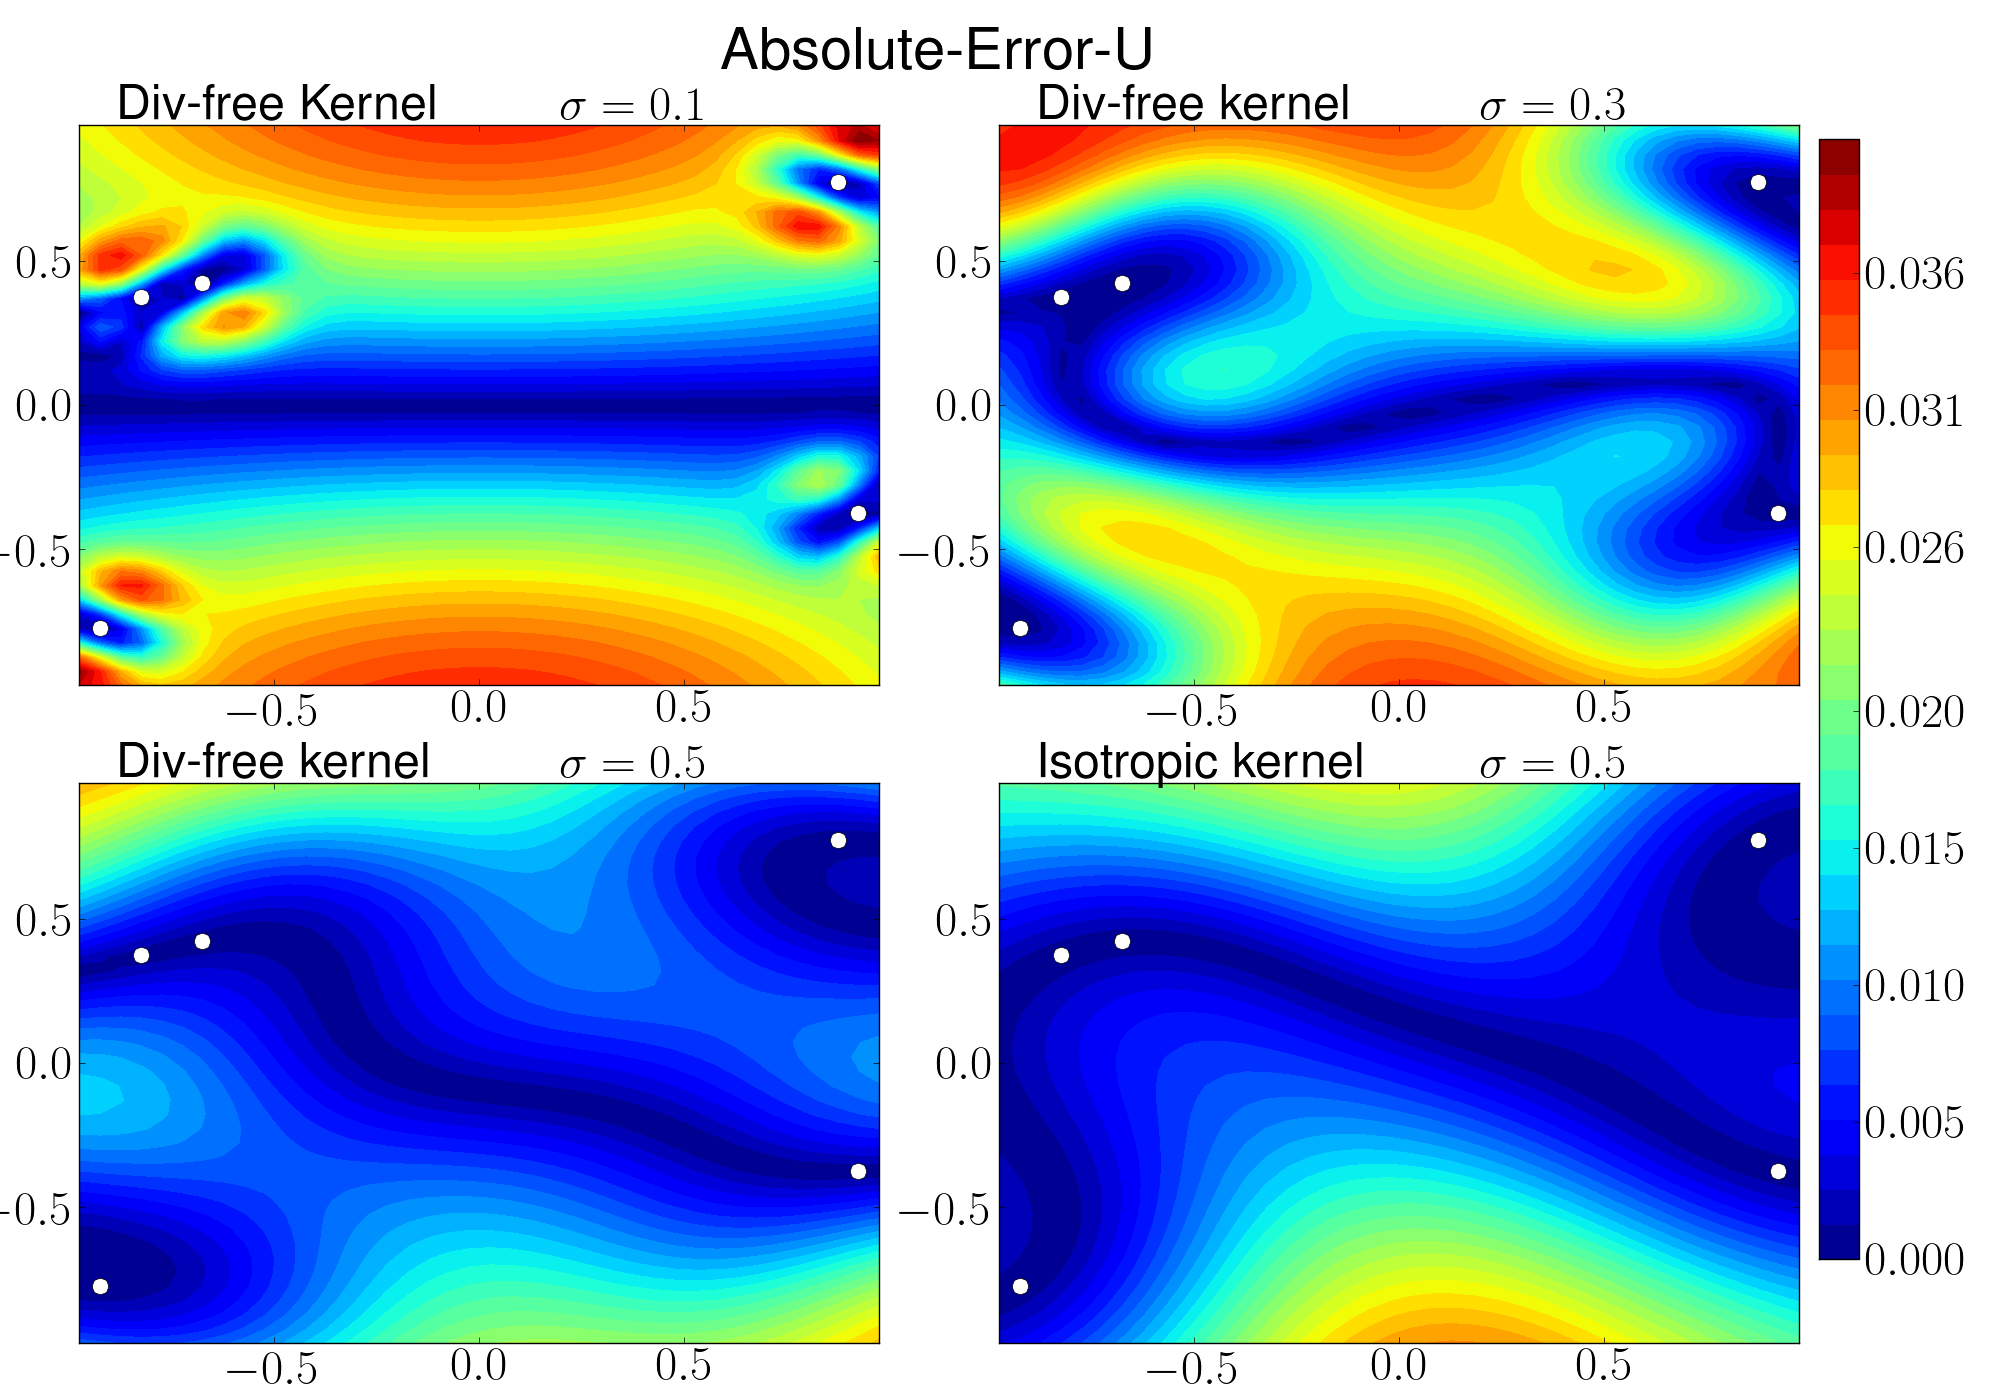
\includegraphics[width=36pc]{plots/Absolute-Error-U-contour.png}
\caption{Absolute error of the zonal velocity component. The white 
dots indicate the location of the observations.}
\label{contour_u}
\end{figure}

\begin{figure}
\noindent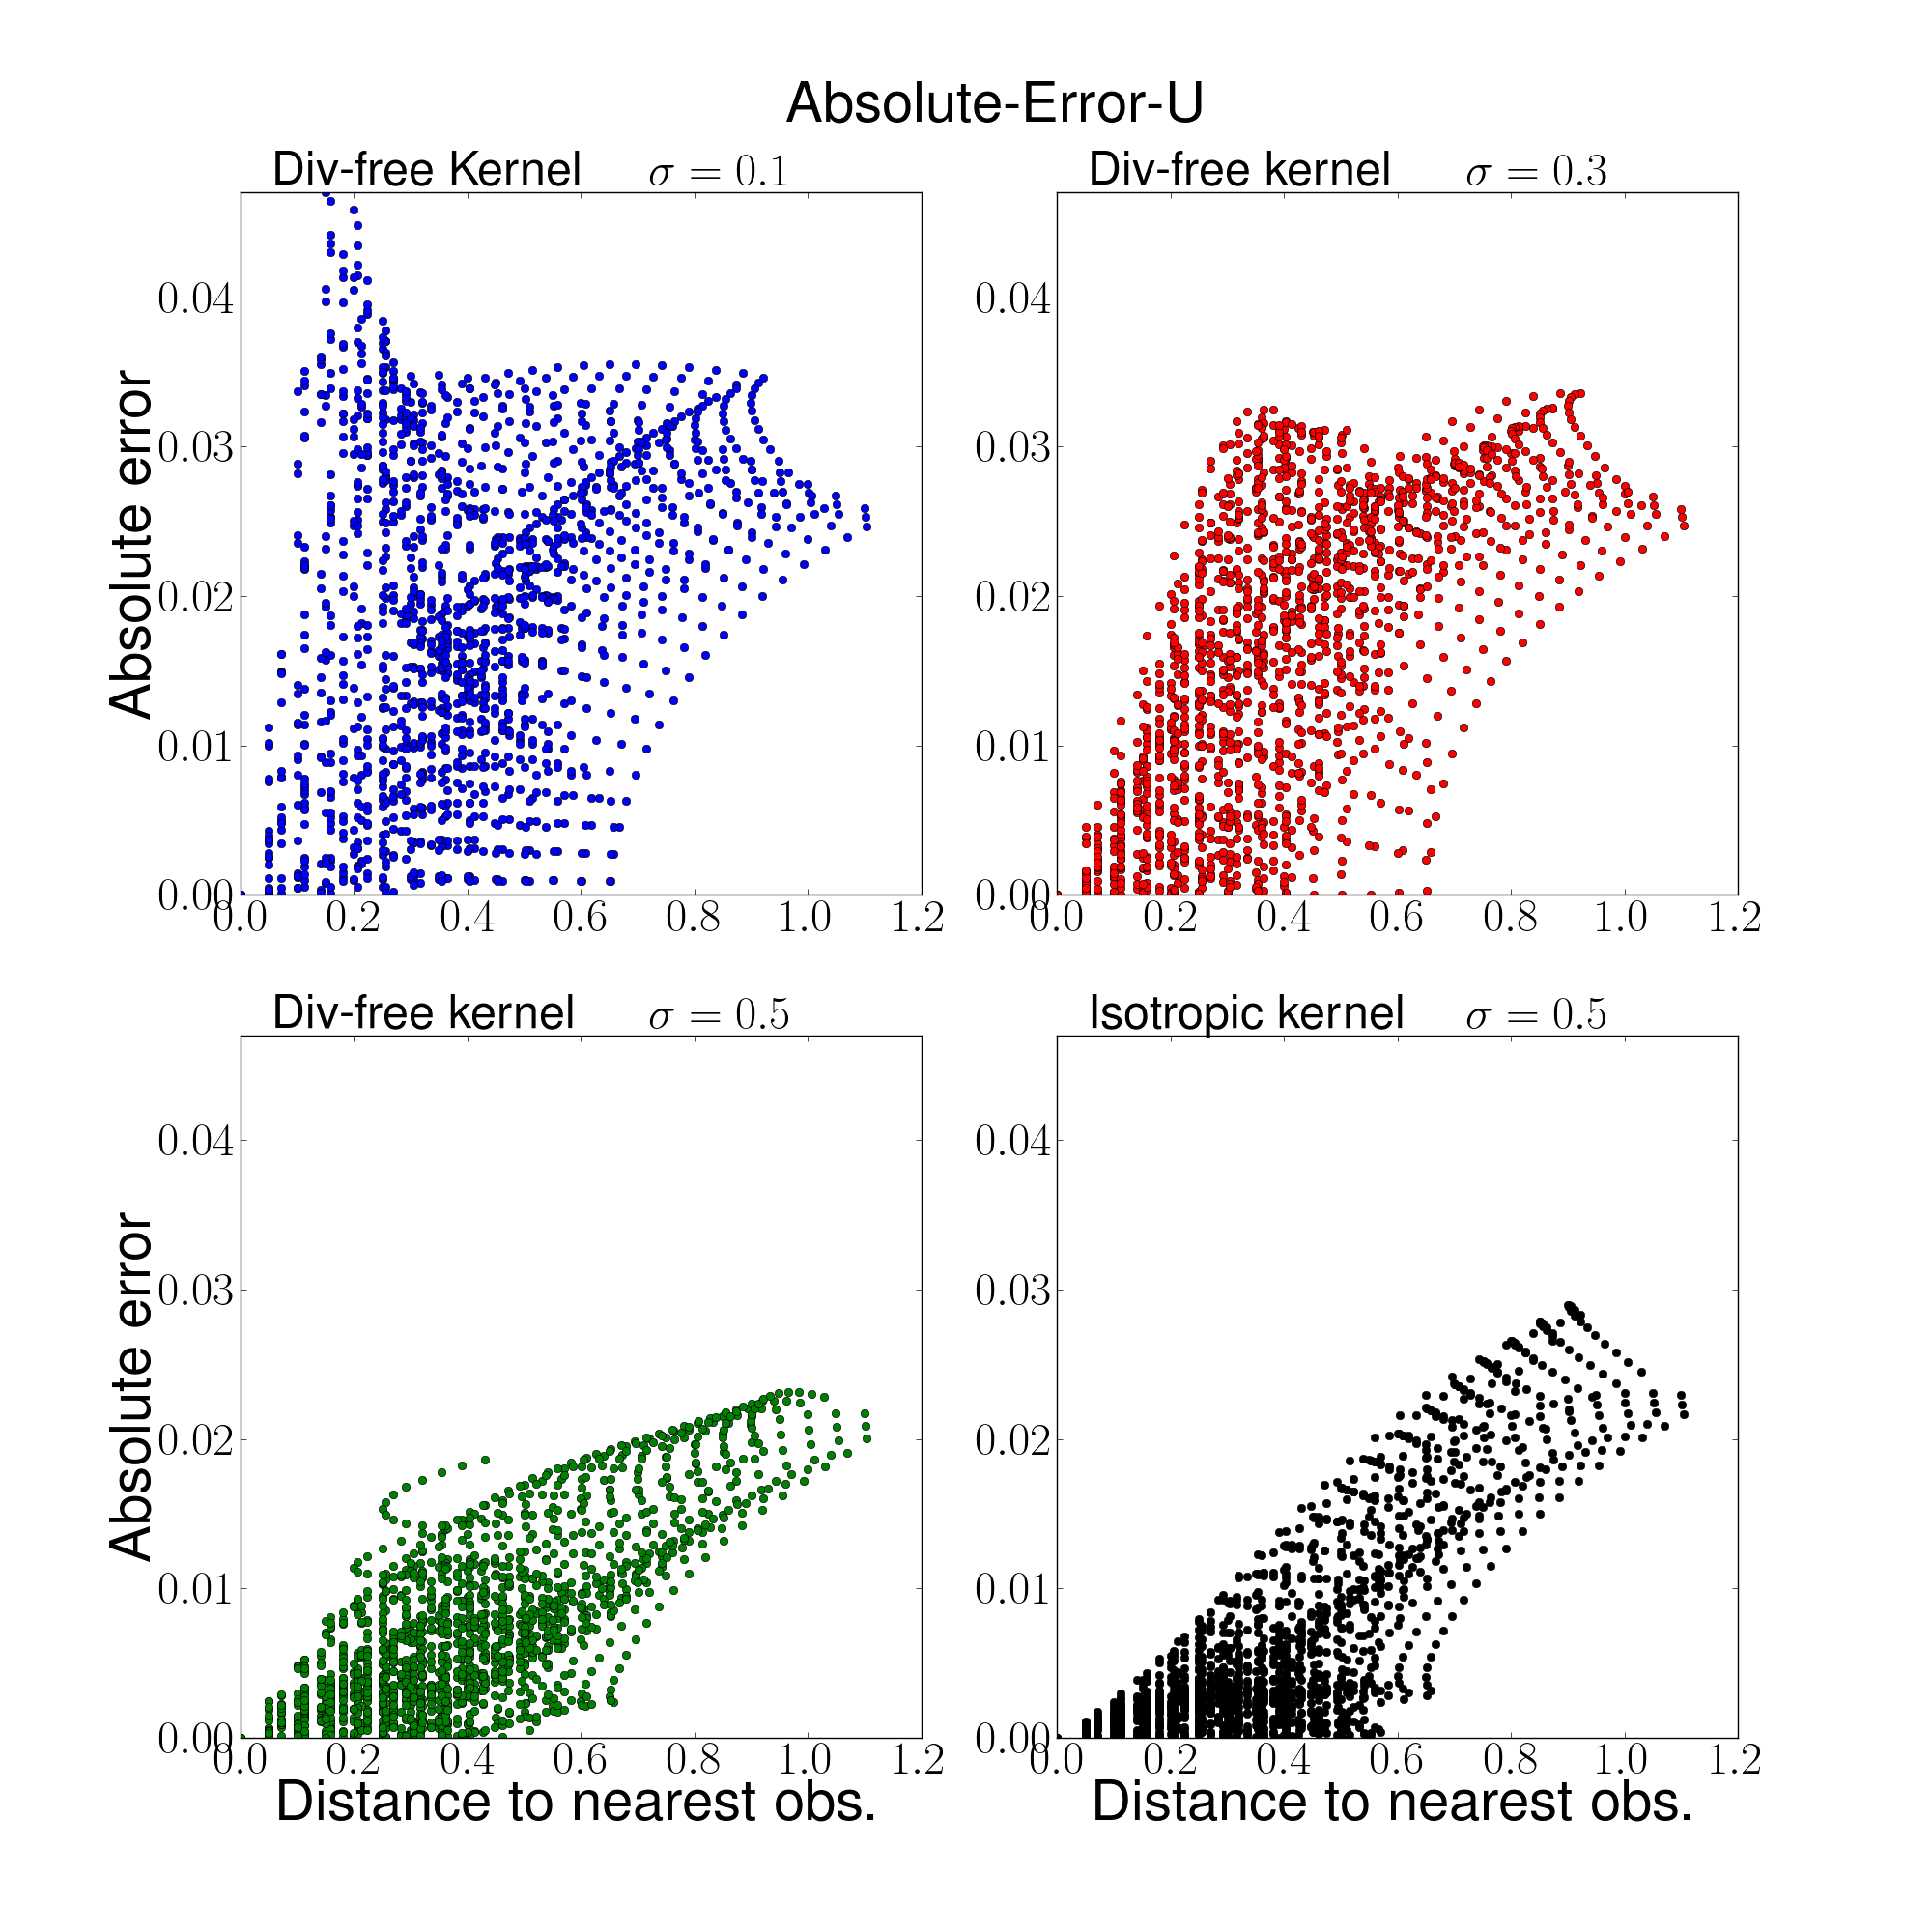
\includegraphics[width=36pc]{plots/Absolute-Error-U-scatter.png}
\caption{Scatter plots of absolute error by distance to nearest observation of 
the zonal velocity component.}
\label{scatter_u}
\end{figure}


\begin{figure}
\noindent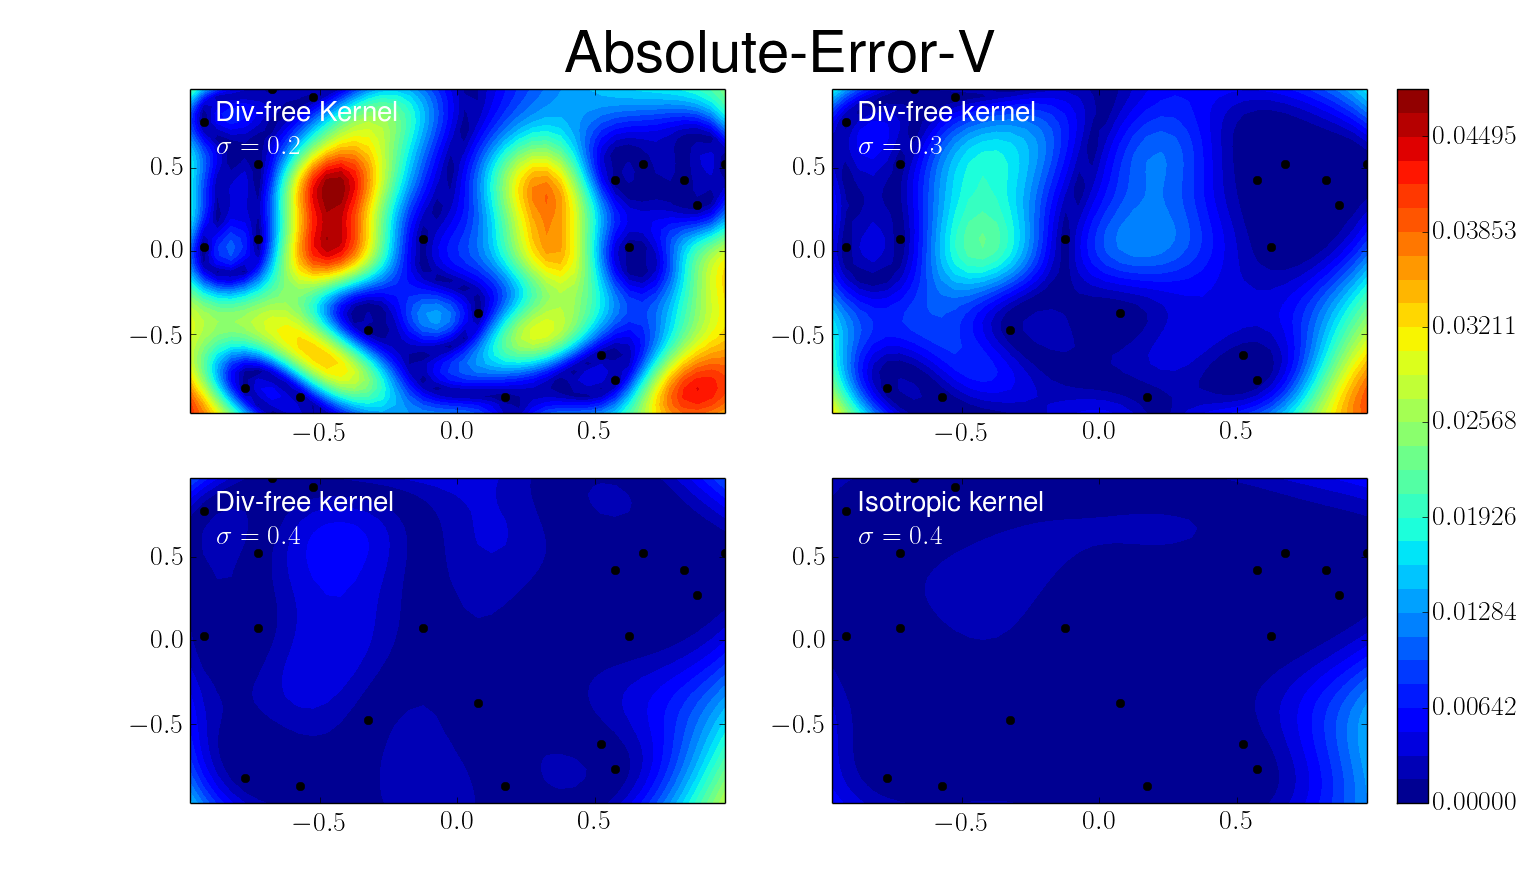
\includegraphics[width=36pc]{plots/Absolute-Error-V-contour.png}
\caption{Same as \ref{contour_u} for the meridional component.  }
\label{contour_v}
\end{figure}

\begin{figure}
\noindent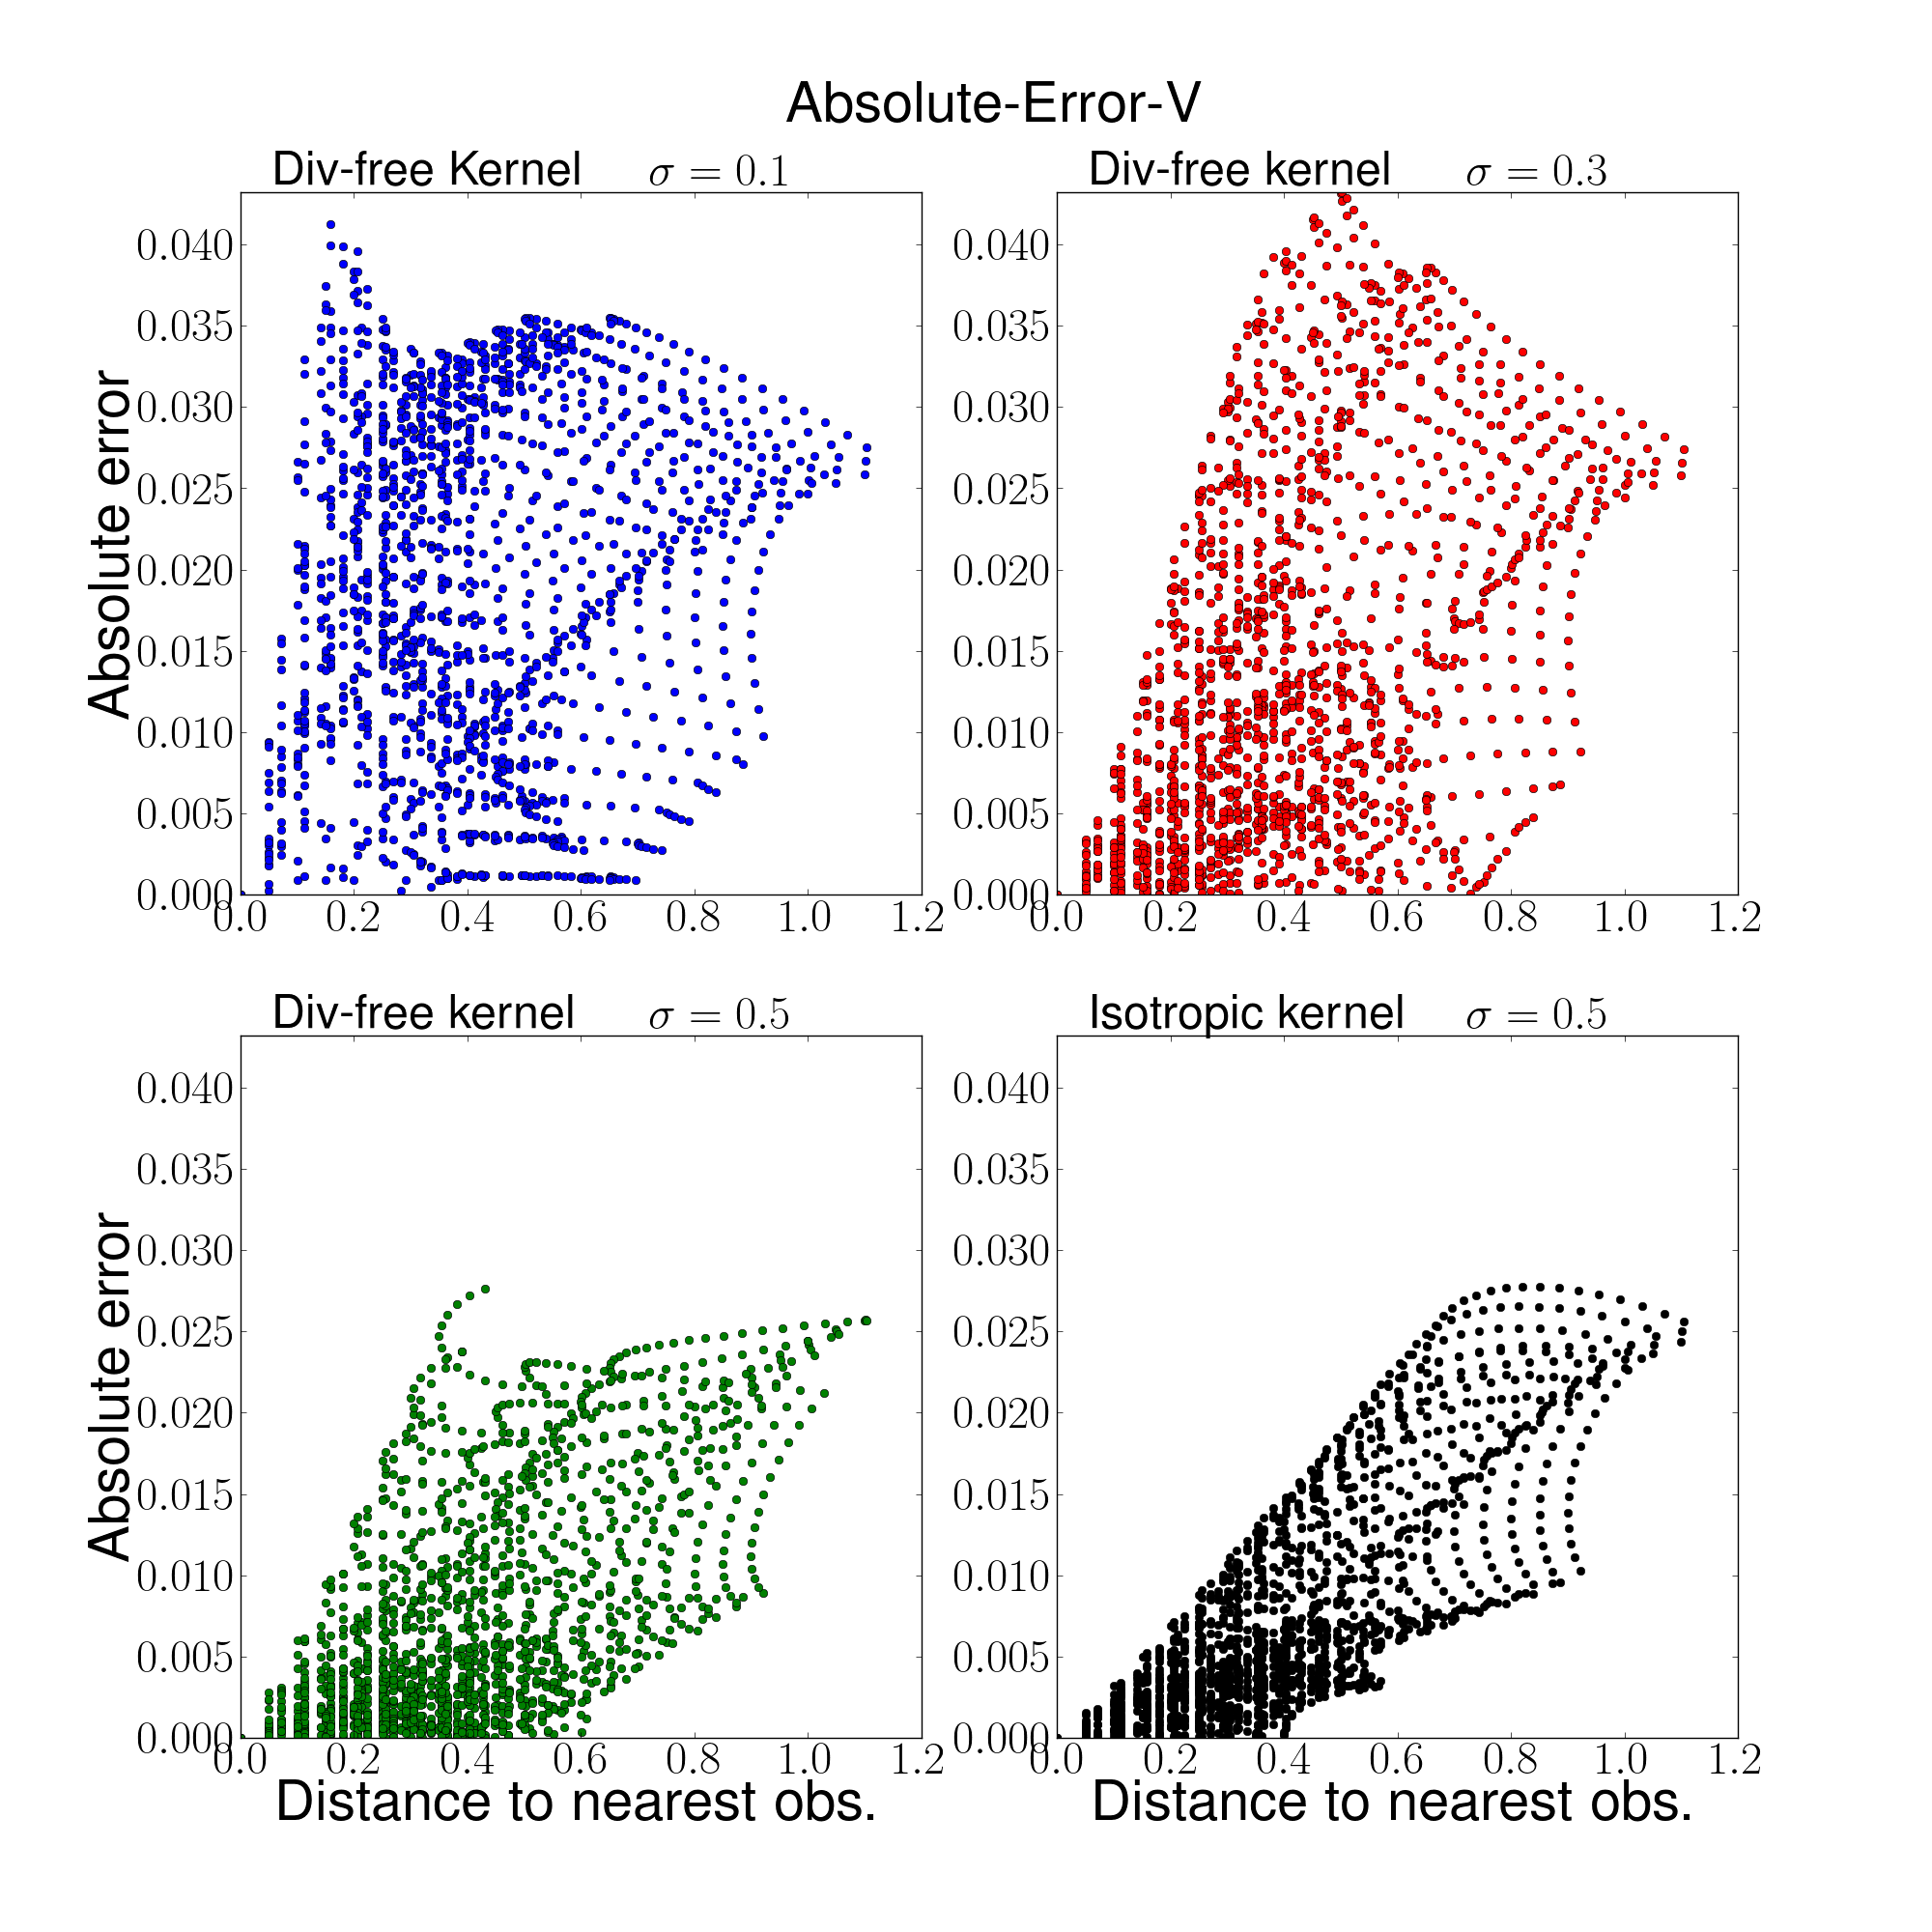
\includegraphics[width=36pc]{plots/Absolute-Error-V-scatter.png}
\caption{Same as Figure \ref{scatter_u} for the meridional component.  }
\label{scatter_v}
\end{figure}

\begin{figure}
\noindent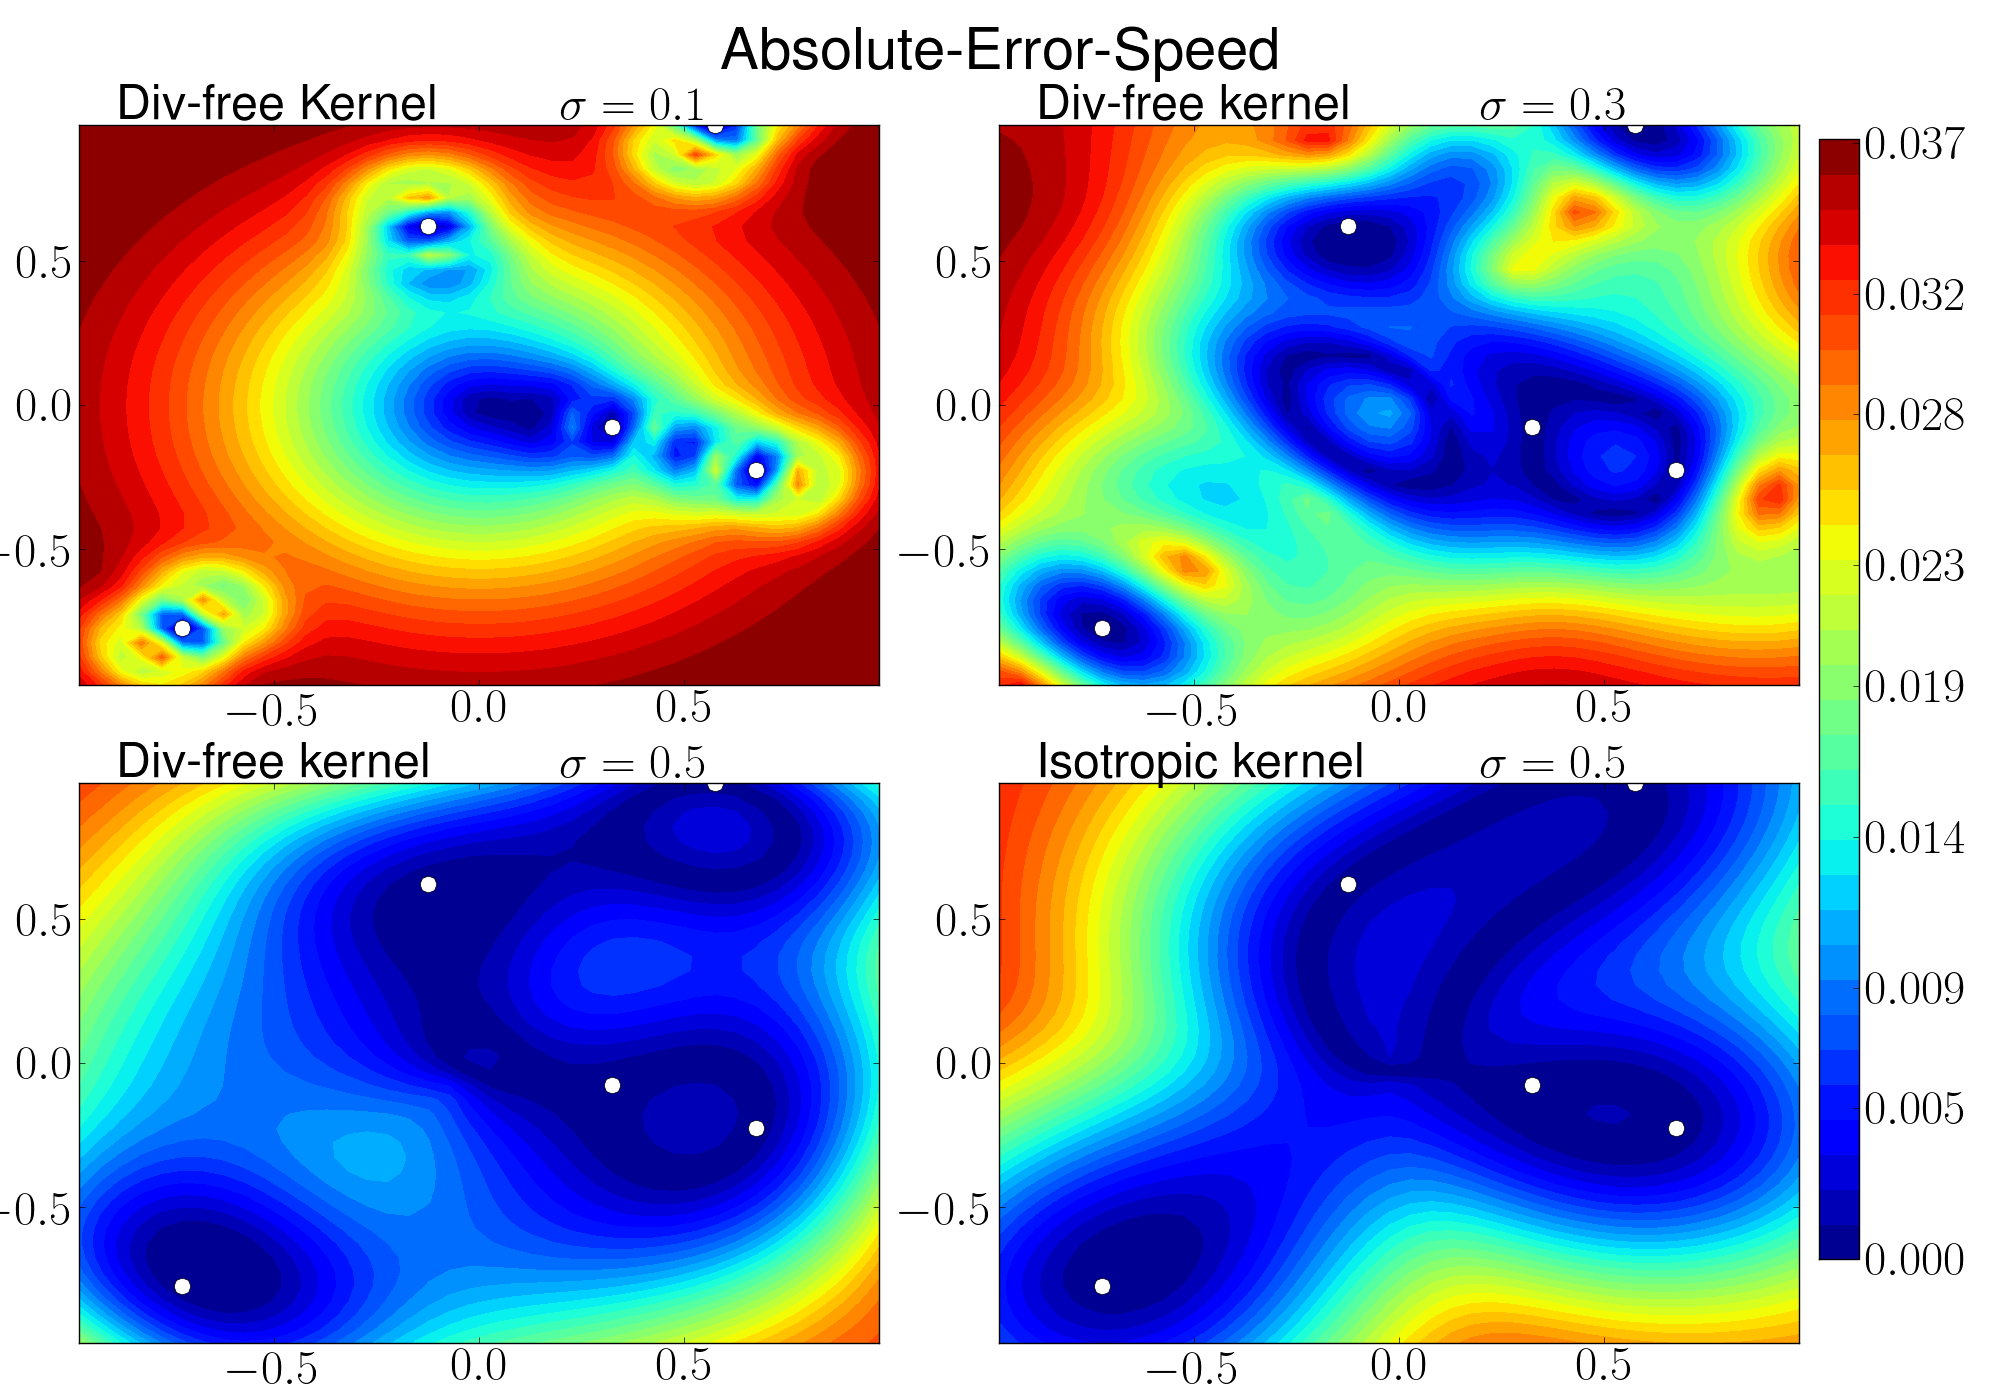
\includegraphics[width=36pc]{plots/Absolute-Error-Speed-contour.png}
\caption{Same as \ref{contour_u} for the absolute velocity. }
\label{contour_speed}
\end{figure}

\begin{figure}
\noindent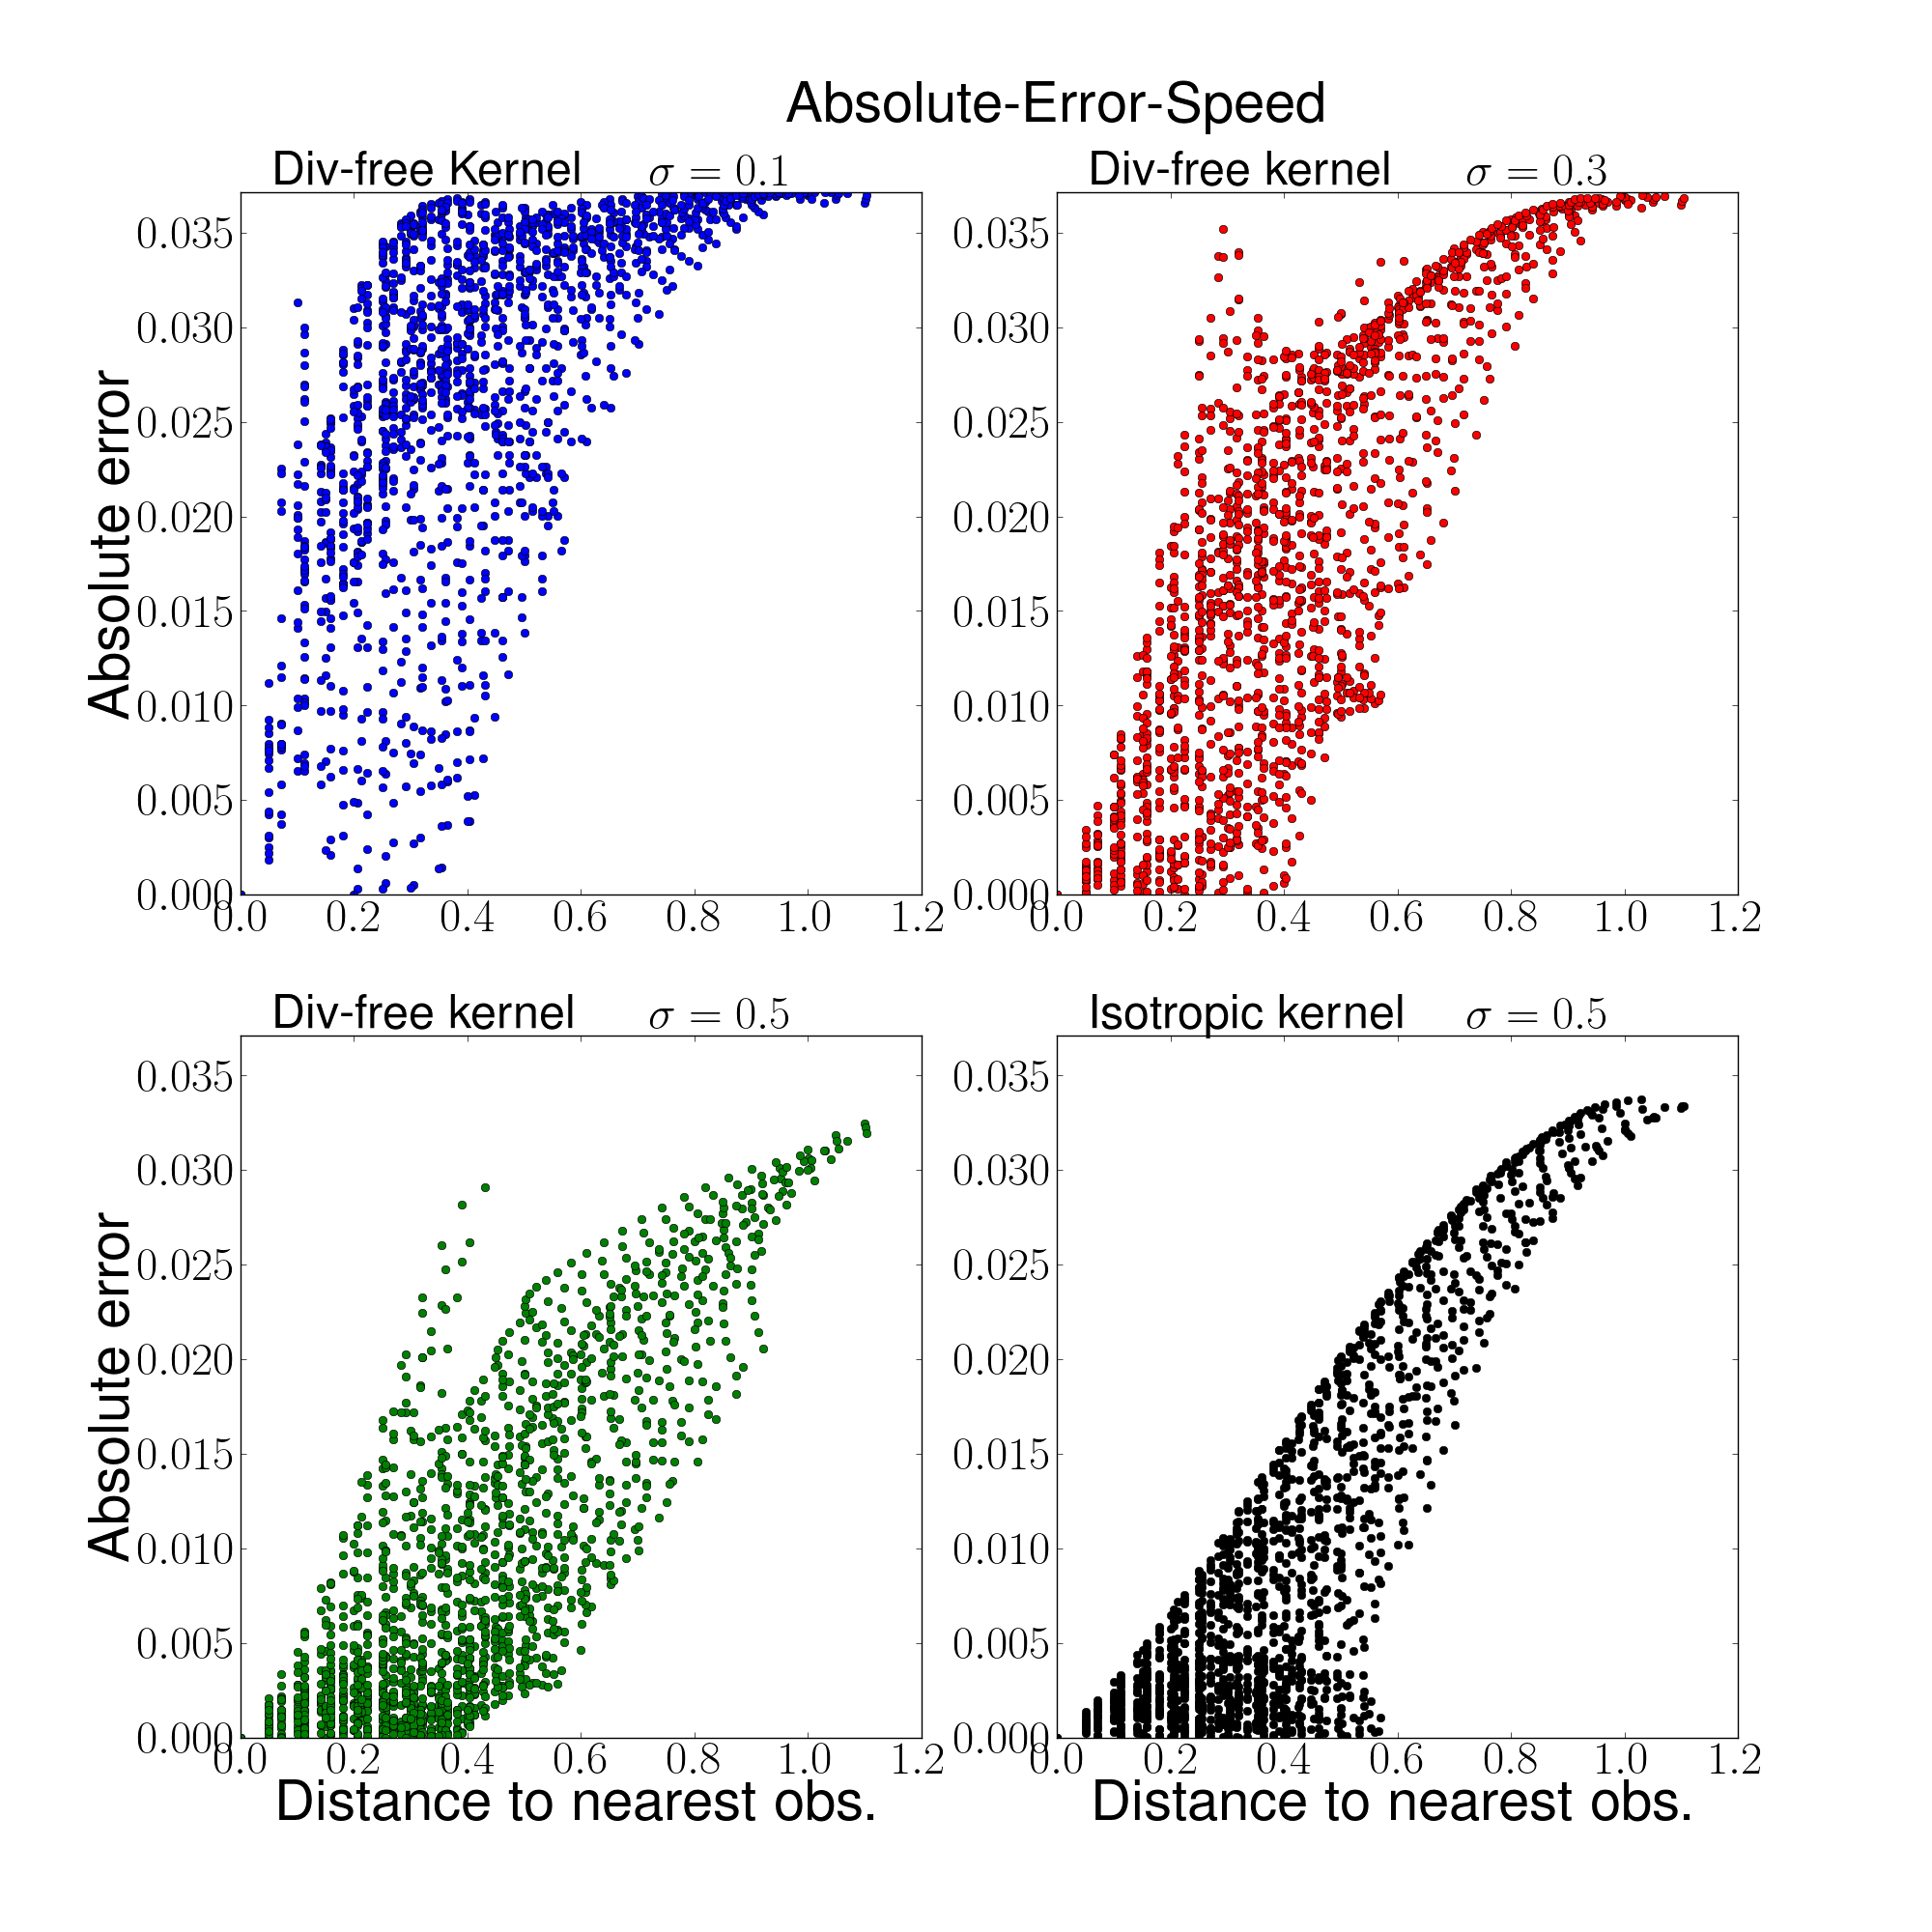
\includegraphics[width=36pc]{plots/Absolute-Error-Speed-scatter.png}
\caption{Same as Figure \ref{scatter_u} for the absolute velocity. }
\label{scatter_speed}
\end{figure}

\begin{figure}
\noindent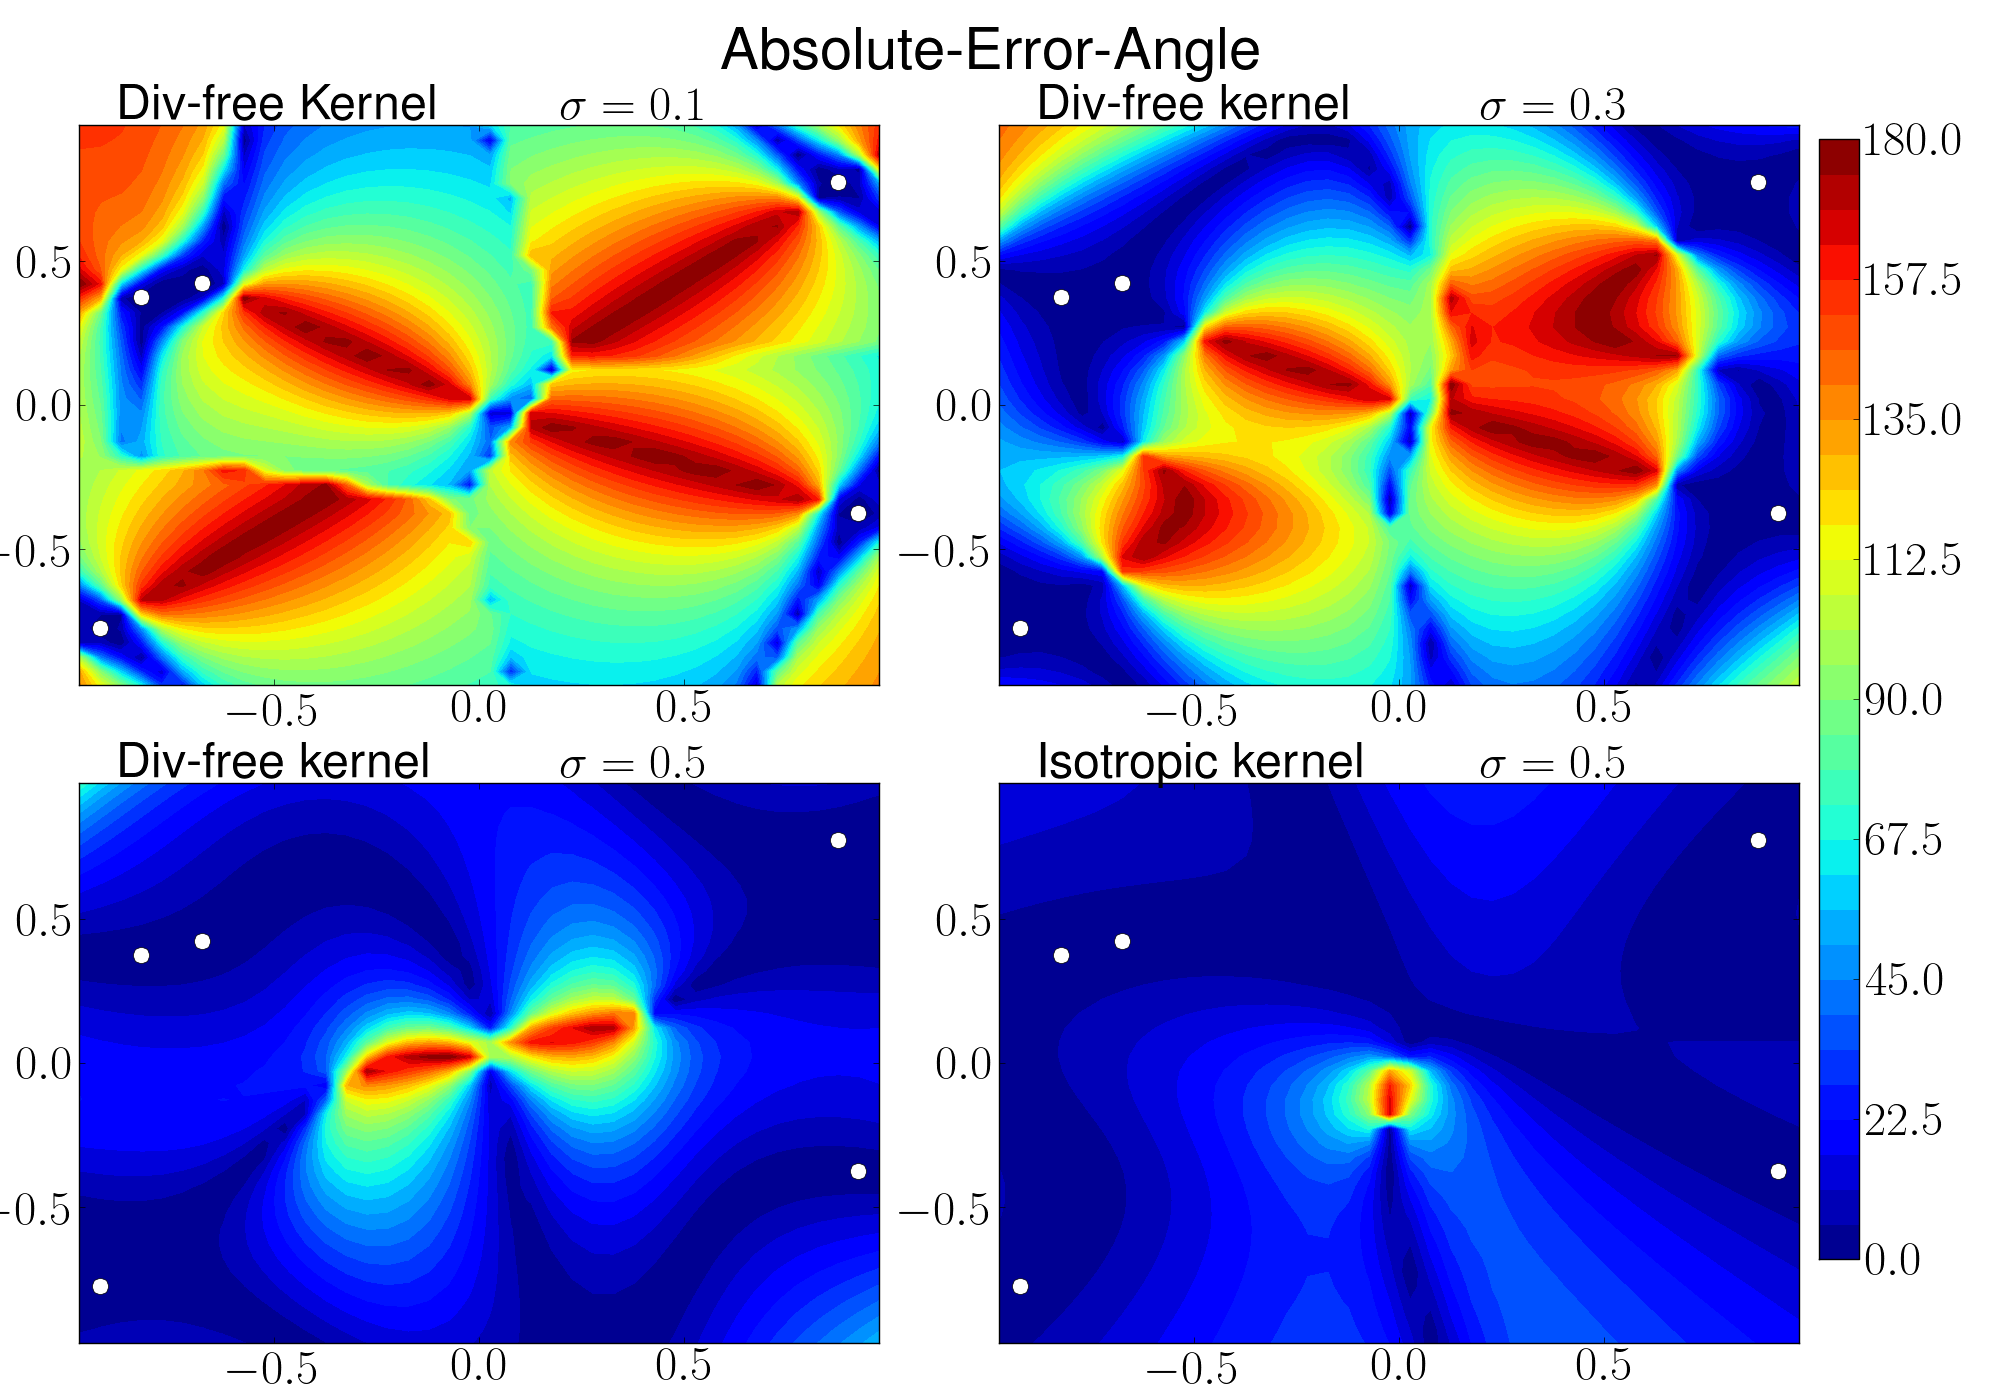
\includegraphics[width=36pc]{plots/Absolute-Error-Angle-contour.png}
\caption{Same as \ref{contour_u} for the direction of the velocity (in degrees). }
\label{contour_angle}
\end{figure}

\begin{figure}
\noindent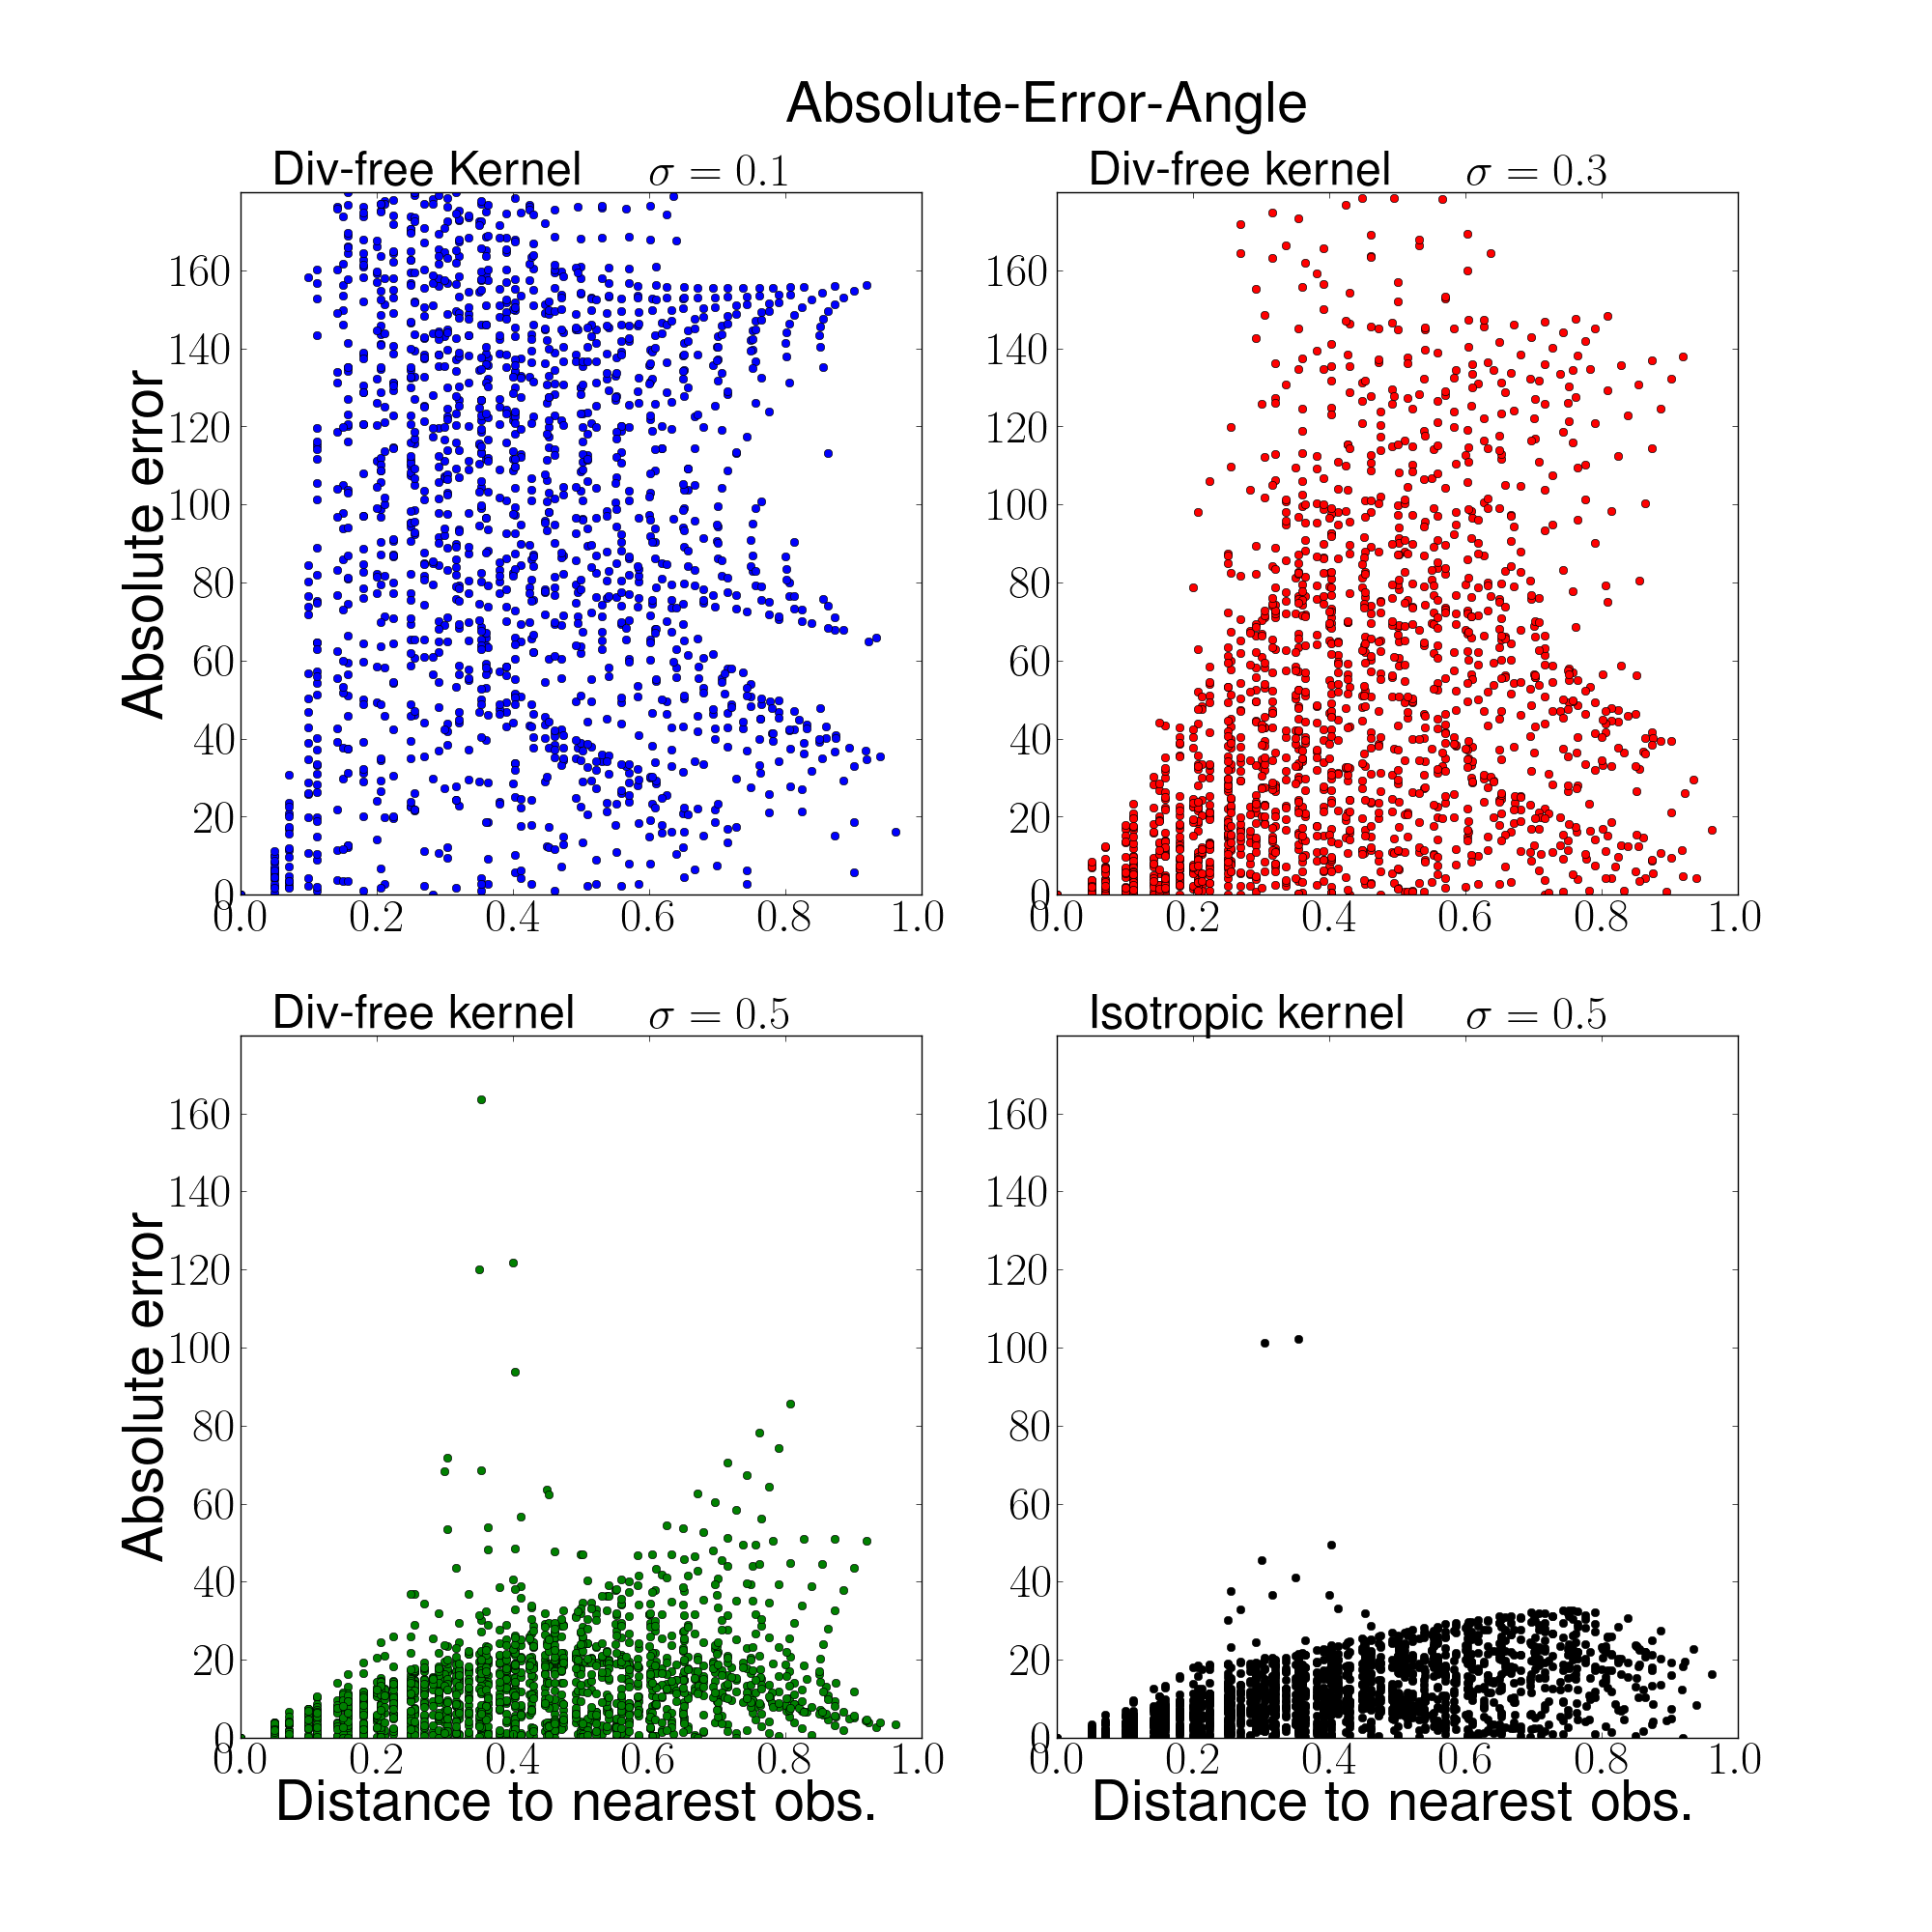
\includegraphics[width=36
pc]{plots/Absolute-Error-Angle-scatter.png}
\caption{Same as Figure \ref{scatter_u} for the direction of the velocity (in degrees). }
\label{scatter_angle}
\end{figure}

\end{document}